\documentclass[a4paper,12pt]{report}

\usepackage[utf8]{inputenc}
\usepackage[T1]{fontenc}
\usepackage[italian]{babel}
\usepackage{geometry}
\usepackage{lmodern}
\usepackage{graphicx}
\usepackage{float}
\usepackage{tabularx}
\usepackage[table]{xcolor}
\usepackage{fancyvrb} 
\usepackage{alltt}
\usepackage{amsmath}
\usepackage{hyperref}

\geometry{margin=1in}

\hypersetup{
    colorlinks=false,
    pdfborder={1 1 1},
    linkbordercolor={1 0 0},
    urlbordercolor={1 0 0},
    citebordercolor={1 0 0},
    pdftitle={Elaborato Basi di Dati},
    pdfauthor={Maisam Noumi, Alessandro Rebosio, Filippo Ricciotti}
}

\usepackage[italian]{cleveref}

\title{
    \vspace*{2cm}
    \Huge\textbf{Agriturismo} \\[0.5cm]
    \LARGE Relazione per il corso di \\[0.2cm]
    \textit{Basi di Dati} \\[2cm]
}

\author{
    \Large
    Maisam Noumi \\
    Alessandro Rebosio \\
    Filippo Ricciotti
}

\date{
    \vspace{1cm}
    \today \\[0.5cm]
    Anno Accademico 2024-2025
}


\begin{document}


\maketitle

\tableofcontents

\chapter{Analisi dei requisiti}
Si ha come obiettivo la realizzazione di un database per la gestione di un agriturismo che offre un'ampia gamma di servizi: ristorazione,
ospitalità, piscina, attività con animali, sport e molto altro.

\section{Intervista}
\textit{L'agriturismo "Campo Verde" offre una vasta gamma di servizi, tra cui ospitalità, ristorazione, piscina, attività con animali
	e sport, e necessita di un sistema integrato per la gestione delle prenotazioni, dei clienti e delle attività.}

\textit{Il sistema dovrà gestire diverse tipologie di servizi, tra cui camere, tavoli al ristorante, lettini in piscina, attività
	con animali e campo da calcio. Ogni servizio avrà regole specifiche: ad esempio, i lettini in piscina sono prenotabili per fasce orarie
	di 2 ore, mentre il campo da calcio può essere prenotato per un'ora o più.}

\textit{Per ogni cliente verranno memorizzati nome, cognome, codice fiscale, indirizzo email e numero di telefono. Al momento della
	registrazione, verrà creato un account personale con credenziali di accesso alla piattaforma. Ogni cliente potrà effettuare prenotazioni
	solo se autenticato, e ogni prenotazione verrà registrata con i relativi dettagli (servizio richiesto, data, orario e numero di partecipanti).}

\textit{I clienti potranno acquistare sia servizi singoli che pacchetti combinati, creati dallo staff o personalizzati in base alle
	loro esigenze. Ogni pacchetto potrà includere più servizi (es. pernottamento + cena + attività con animali) e avrà un prezzo
	specifico, con eventuali sconti applicabili in base alla stagione o a promozioni speciali.}

\textit{Ogni prenotazione verrà confermata via email, con la possibilità di modificarla o cancellarla entro un certo termine. In
	caso di mancata presentazione senza preavviso, potrà essere applicata una penale. Le prenotazioni per eventi speciali (come tornei o cene a tema)
	richiederanno spesso un acconto non rimborsabile.}

\textit{L'agriturismo terrà traccia di tutte le prenotazioni effettuate dai clienti, mantenendo uno storico che permetterà
	di analizzare le preferenze e di proporre offerte personalizzate. I clienti potranno lasciare recensioni per ogni servizio utilizzato, valutandolo
	con un voto da 1 a 5 stelle e aggiungendo un commento. Le recensioni verranno moderate dallo staff e potranno essere utilizzate per
	migliorare i servizi offerti.}

\textit{Il sistema permetterà anche la gestione degli eventi organizzati dall'agriturismo, come tornei di calcio o laboratori con animali. Per ogni
	evento sarà possibile definire il numero massimo di partecipanti, il prezzo e le date disponibili. I clienti potranno iscriversi agli eventi direttamente
	dalla piattaforma, ricevendo una conferma e i dettagli organizzativi.}

\textit{Lo staff dell'agriturismo avrà accesso a una dashboard che mostrerà in tempo reale lo stato delle prenotazioni, l'occupazione delle
	camere e dei servizi, e le recensioni ricevute. Potranno generare report periodici per analizzare l'andamento delle prenotazioni, le preferenze dei clienti e
	l'efficacia delle promozioni. Inoltre, il sistema supporterà la gestione di account multipli per lo staff, con diversi livelli di accesso in base al
	ruolo (es. receptionist, responsabile del ristorante, gestore della piscina).}

\section{Estrazione dei concetti principali}
Dall'analisi svolta emergono le principali entità che il sistema dovrà gestire: \textbf{Cliente}, \textbf{Servizio}, \textbf{Prenotazione},
\textbf{Pacchetto}, \textbf{Evento}, \textbf{Recensione} e \textbf{Staff}.

Ogni \textbf{Cliente} potrà registrarsi fornendo i seguenti attributi: \newline \underline{nome}, \underline{cognome}, \underline{codice fiscale},
\underline{email} e \underline{numero di telefono}. All'atto della registrazione, verrà creato un account contenente \underline{username} e \underline{password}. Solo i clienti
autenticati potranno effettuare prenotazioni. Ogni cliente avrà accesso al proprio \underline{storico prenotazioni} e potrà lasciare recensioni.

I \textbf{Servizi} gestiti comprendono: \underline{camere}, \underline{tavoli ristorante}, \newline \underline{lettini piscina}, \underline{attività con
	animali} e \underline{campo da calcio}. Ogni servizio presenta regole specifiche: ad esempio, i lettini in piscina sono prenotabili a fasce orarie di
due ore, mentre il campo da calcio è prenotabile per una o più ore. Per ciascun servizio devono essere definiti \underline{orari}, \underline{capacità massima},
\underline{durata prenotabile} e \underline{penali in caso di cancellazione}.

La \textbf{Prenotazione} sarà associata a un cliente e a uno o più servizi, e includerà \underline{data}, \underline{orario}, \underline{numero di
	partecipanti} e \underline{stato}. La cancellazione sarà possibile secondo i termini previsti (es. 48 ore per le camere, 24 per servizi a tempo). In caso di
mancata presentazione, potrà essere applicata una \underline{penale}, mentre per eventi speciali sarà richiesto un \underline{acconto non rimborsabile}.

Il sistema gestirà anche \textbf{Pacchetti}, ovvero combinazioni \newline di più servizi, con un \underline{prezzo complessivo},
eventuali \underline{sconti promozionali} e possibilità \newline di \underline{personalizzazione}. I pacchetti potranno essere creati dallo staff o richiesti dai clienti.

Per quanto riguarda gli \textbf{Eventi}, come tornei o laboratori, saranno definiti con \underline{nome}, \newline \underline{descrizione}, \underline{data},
\underline{prezzo}, \underline{numero massimo di partecipanti} e, se necessario, \underline{acconto}. I clienti potranno iscriversi online e riceveranno conferma via email.

Le \textbf{Recensioni} potranno essere lasciate dai clienti solo dopo aver usufruito di un servizio. Ogni recensione includerà
una \underline{valutazione da 1 a 5 stelle} e un \underline{commento testuale}. Le recensioni verranno \underline{moderate} dallo staff prima della pubblicazione.

Lo \textbf{Staff} accederà al sistema tramite un \underline{account personale} con \underline{ruolo} definito (es. receptionist, gestore piscina). Tramite
una \underline{dashboard}, lo staff potrà monitorare in tempo reale le \underline{prenotazioni}, lo \underline{stato di occupazione dei servizi} e le
\underline{recensioni}. Il sistema permetterà inoltre la \underline{generazione di report} statistici sull'attività dell'agriturismo.


\chapter{Preogettazione concettuale}
In questo capitolo presenteremo lo schema ER, partendo da una versione iniziale e migliorandola passo dopo passo ad arrivare a quella
definitiva, attraverso dei raffinamenti.

\section{Schema scheletro}
Dopo aver eseguito l'analisi del dominio iniziale, abbiamo creato uno schema di base con le entità e le relazioni principali,
che sarà poi perfezionato nei passaggi successivi.
\begin{figure}[H]
	\centering
	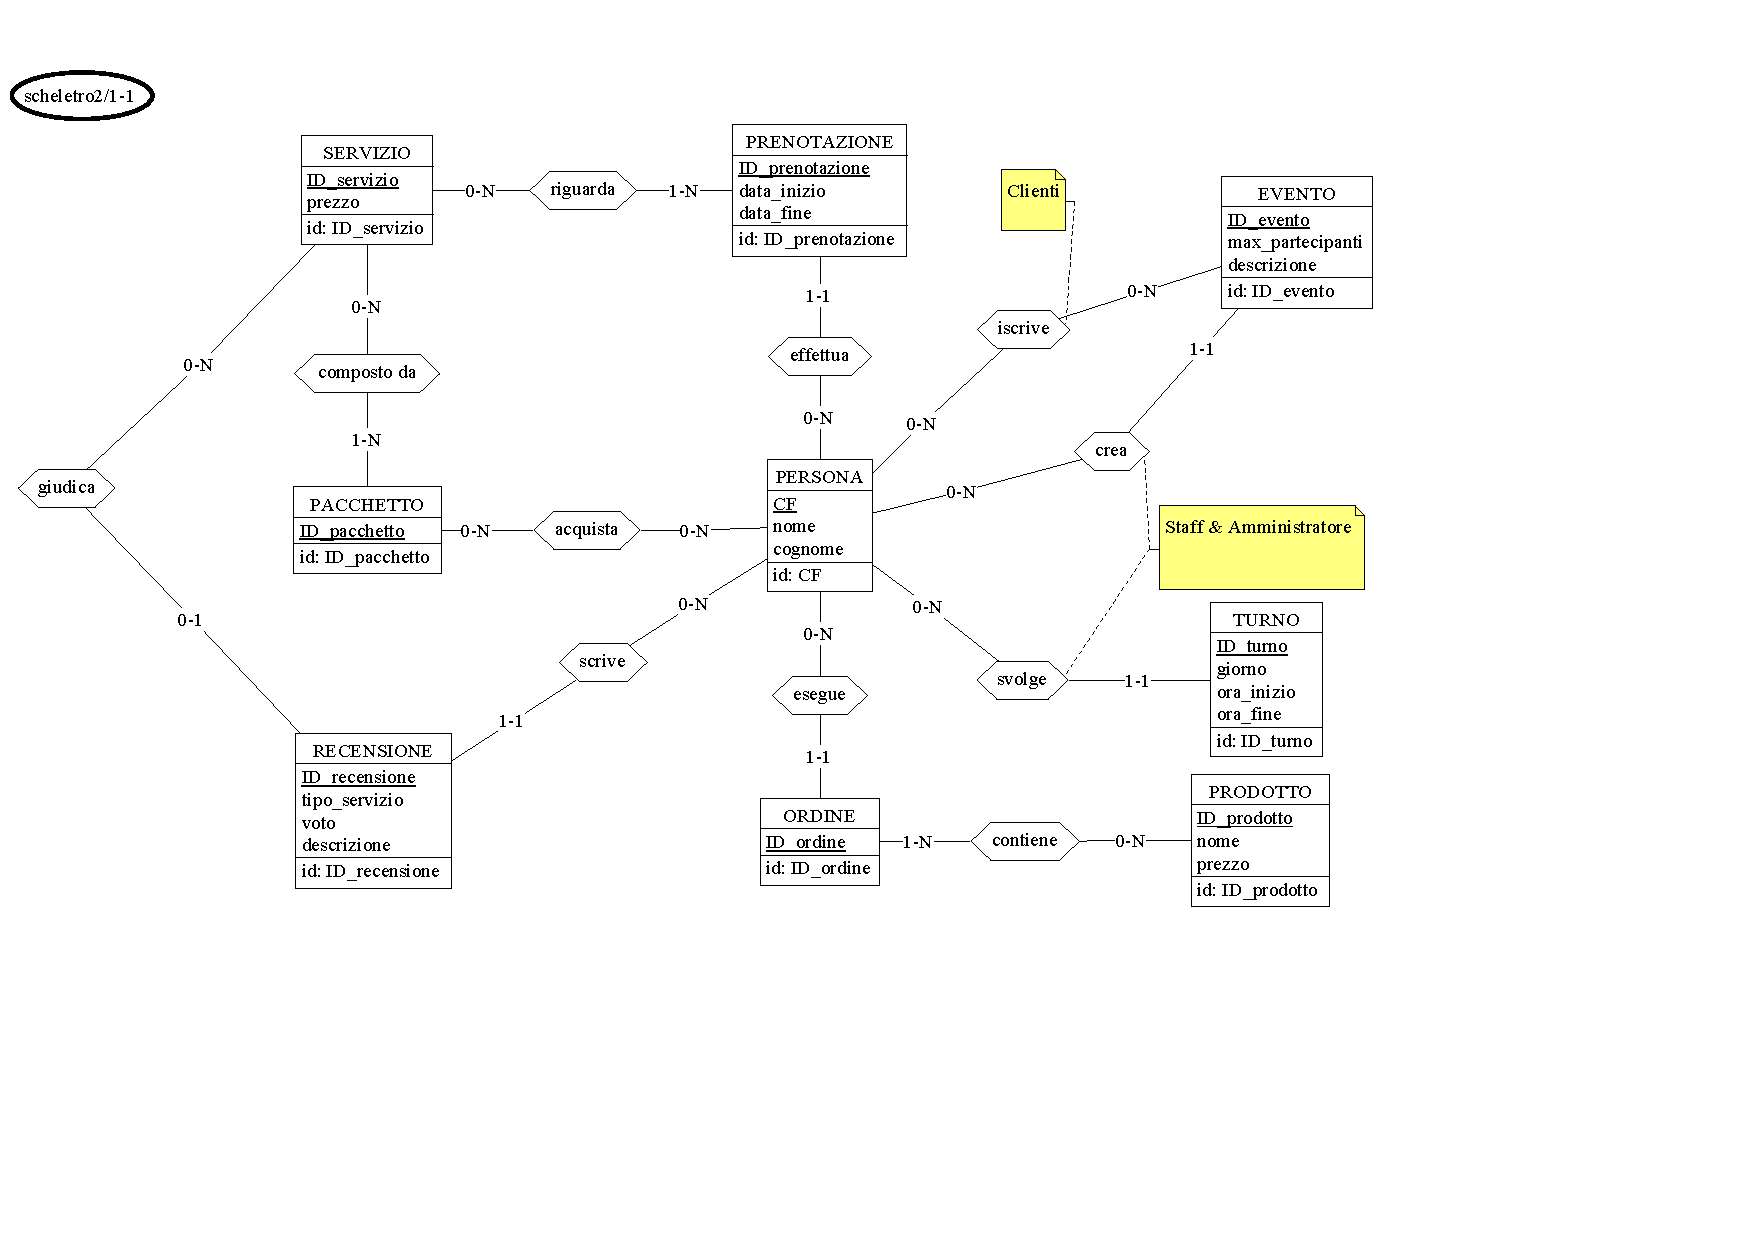
\includegraphics[width=\textwidth, trim=0 100pt 150pt 0 , clip]{./pdf/scheletro.pdf}
	\caption{Schema ER scheletro (versione iniziale)}
	\label{fig:schema-scheletro}
\end{figure}

\section{Raffinamenti proposti}
\subsection{Utente e Dipendente}
Nel modello concettuale iniziale la \textbf{Persona} raggruppava tutte le possibili interazioni con il sistema: iscrizione, creazione
di eventi, acquisto di pacchetti, prenotazioni, ordini e recensioni. Questo approccio, sebbene corretto dal punto di vista logico, risultava poco chiaro
perché attribuiva a un'unica entità responsabilità molto eterogenee.

\vspace{\baselineskip}
Per migliorare la rappresentazione è stato introdotto un raffinamento mediante generalizzazione/specializzazione: la superclasse
\textbf{Persona} è stata mantenuta per raccogliere gli attributi comuni (CF, nome, cognome), mentre le funzionalità specifiche sono state assegnate
ai sottotipi \textbf{Cliente} e \textbf{Dipendente}.

\vspace{\baselineskip}
La relazione \textbf{ospita} tra \textbf{Utente} e \textbf{Persona} ci permette di associare ad un utente più ospiti, evitando di dover creare un account utente per ogni cliente, un utile comodità nei casi dei gruppi famigliari.


\vspace{\baselineskip}
In questo modo i clienti gestiscono attività come acquisti, recensioni, ordini e iscrizioni agli eventi, mentre
i dipendenti si occupano della creazione degli eventi e della gestione dei servizi. Tale raffinamento migliora
la chiarezza semantica del modello, riduce le ambiguità e riflette meglio la separazione dei ruoli reali all'interno
del dominio applicativo.

\begin{figure}[H]
	\centering
	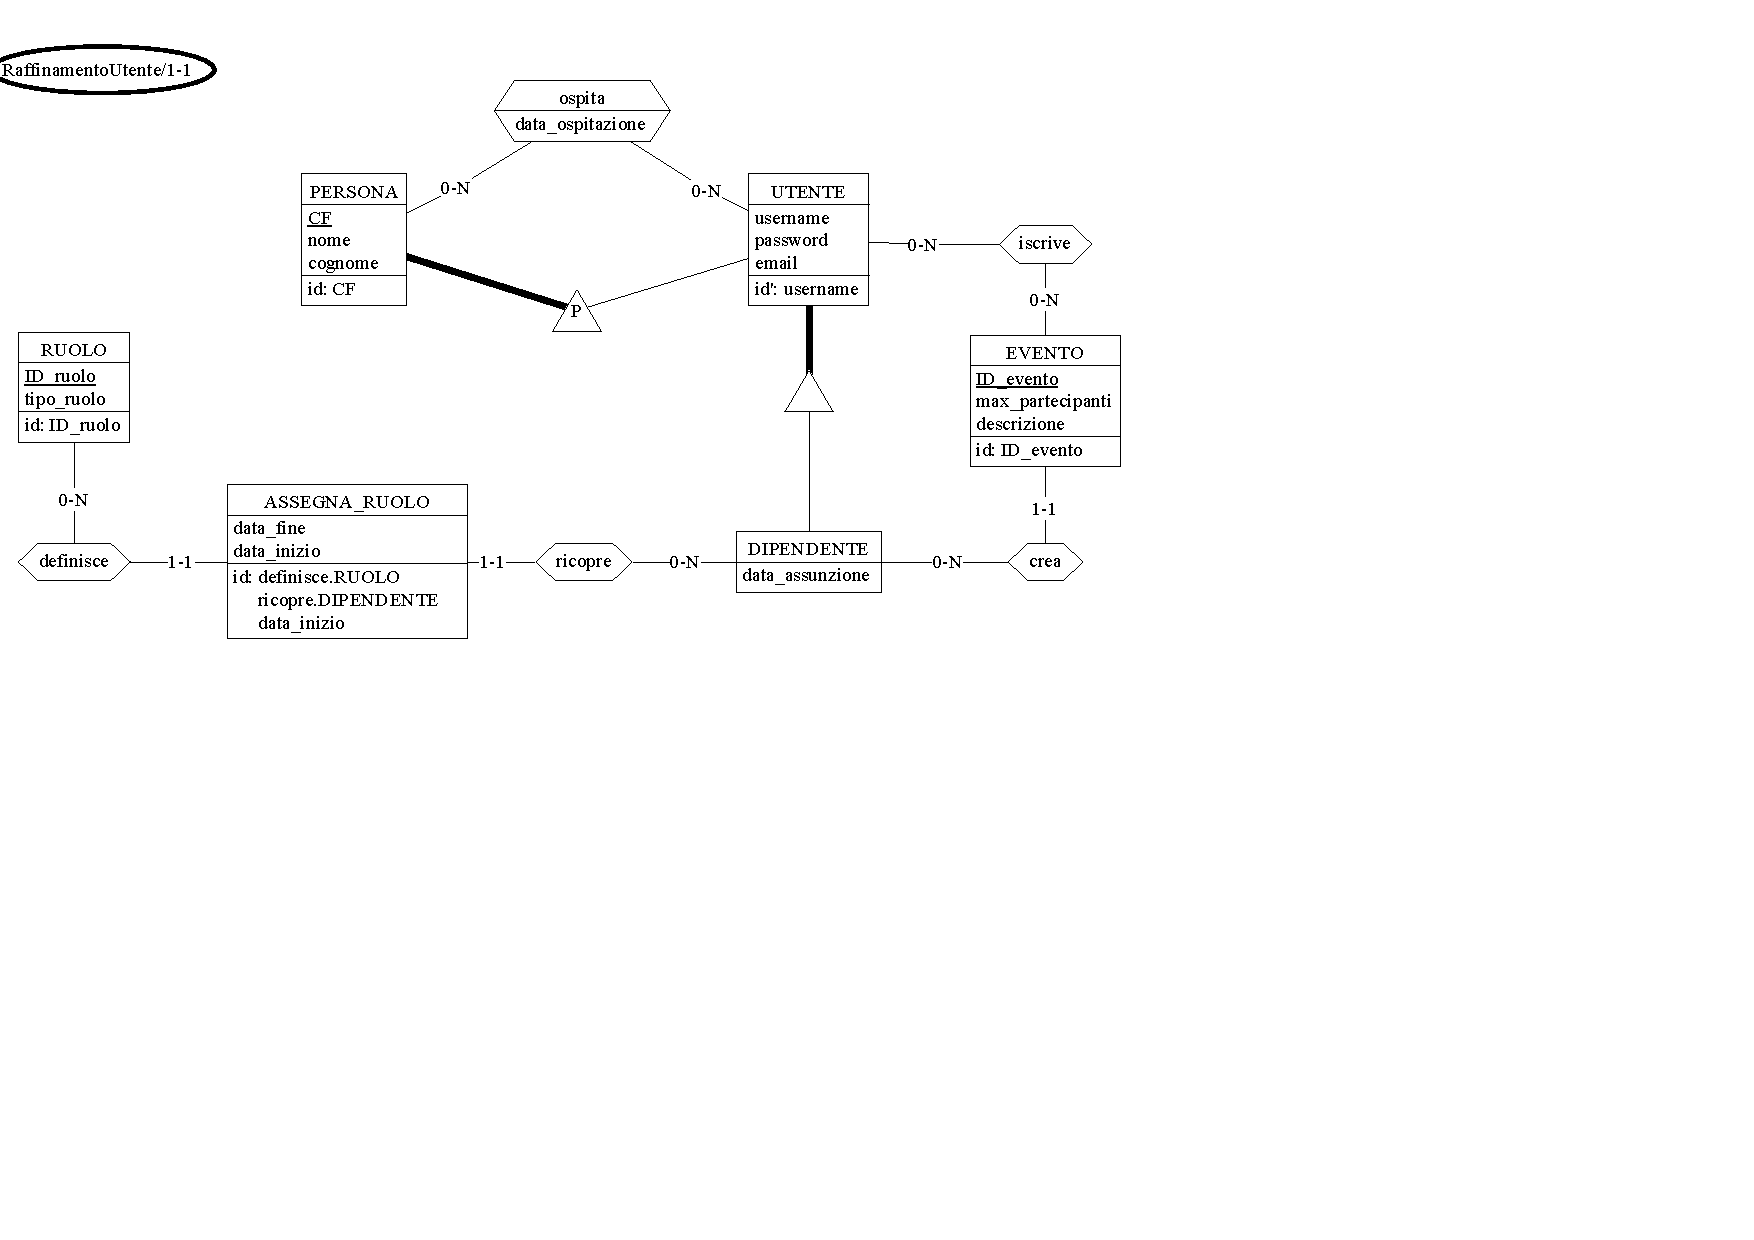
\includegraphics[width=\textwidth, trim=0 250pt 300pt 0, clip]{./pdf/raffinamento utente.pdf}
	\caption{Schema ER, raffinamento utente}
	\label{fig:raffinamento-utente}
\end{figure}

\newpage

\subsection{Ruolo e Turno}
Nel modello concettuale iniziale i ruoli dei dipendenti erano descritti in maniera statica:
un \textbf{Dipendente} poteva ricoprire uno o più \textbf{Ruoli}, ma non era possibile rappresentare
in modo chiaro la distribuzione temporale delle attività lavorative.

\vspace{\baselineskip}
Per migliorare la rappresentazione è stato introdotto un raffinamento attraverso
l'aggiunta dell'entità \textbf{Turno}, caratterizzata da attributi come giorno della settimana,
orario di inizio e fine, ed una descrizione testuale. In questo modo diventa possibile
modellare i turni di lavoro ricorrenti e collegarli direttamente ai ruoli che li richiedono.

\vspace{\baselineskip}
La relazione molti-a-molti tra \textbf{Ruolo} e \textbf{Turno} consente di esprimere sia il fatto
che un ruolo può prevedere più turni (ad esempio il ruolo di cameriere con turni mattutini e serali),
sia che un turno possa essere condiviso tra più ruoli (ad esempio un turno diurno valido sia
per i camerieri che per i receptionist).

Questa scelta arricchisce la chiarezza semantica del modello, riflette la gestione organizzativa reale
e fornisce maggiore flessibilità nella pianificazione delle attività.

\begin{figure}[H]
	\centering
	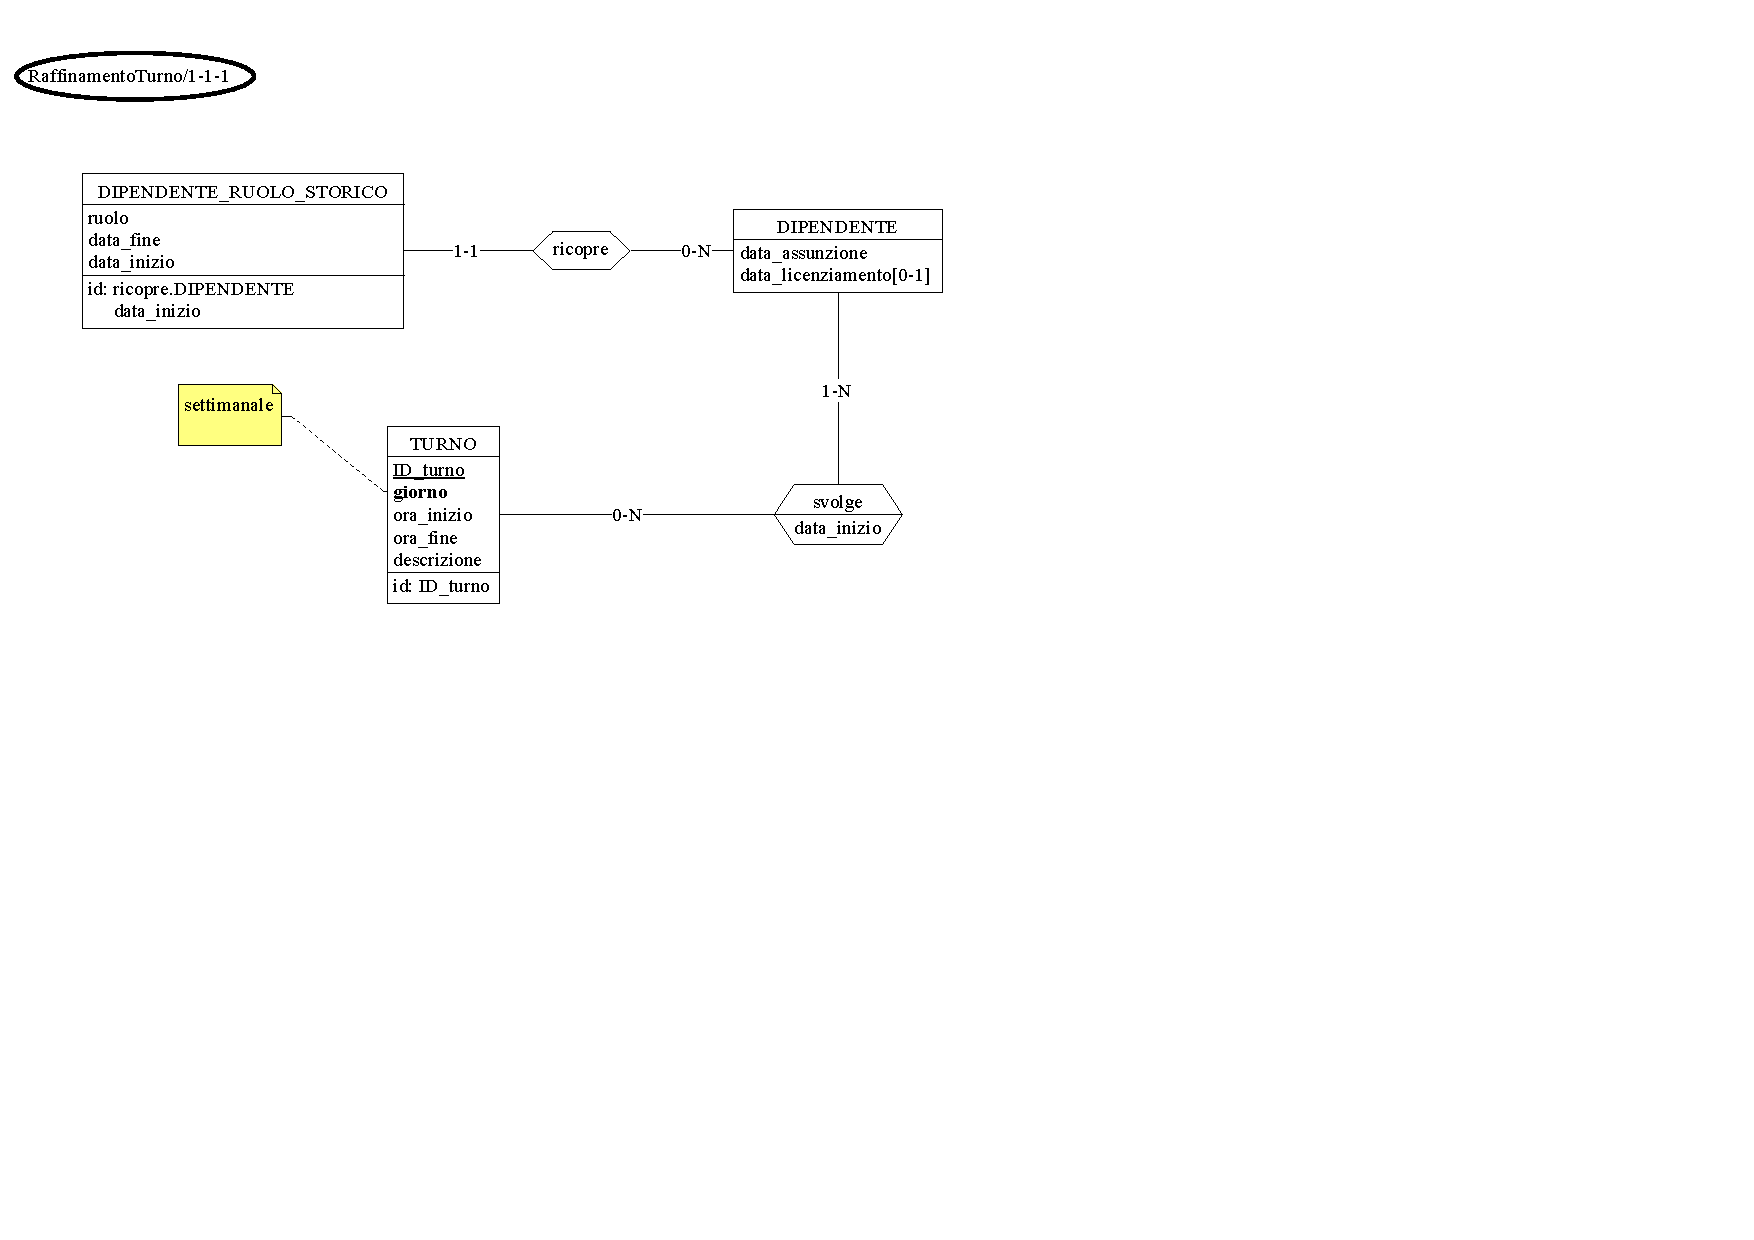
\includegraphics[width=\textwidth, trim=0 250pt 375pt 0, clip]{./pdf/raffinamento turno.pdf}
	\caption{Schema ER, raffinamento turno}
	\label{fig:raffinamento-turno}
\end{figure}

\newpage

\subsection{Servizi/Prenotazioni e Pacchetti}
Nel modello iniziale i diversi tipi di servizi (camere, tavoli, lettini, campi da gioco, attività con animali) potevano essere
rappresentati come entità distinte, con il rischio però di ridondanza e frammentazione dei dati.

\vspace{\baselineskip}
Con il raffinamento si è introdotta una \textbf{generalizzazione}: è stata creata la superclasse \textbf{Servizio}, che raccoglie gli attributi comuni (ID\_servizio,
prezzo, tipo\_servizio, status), mentre ciascuna tipologia specifica di servizio (Camera, Tavolo, Lettino, Campo da gioco,
Attività con animali) è modellata come sottoclasse.

\vspace{\baselineskip}
Inoltre, è stato introdotto il legame con l'entità \textbf{Prenotazione}, che consente di registrare le informazioni su data di inizio
e fine e di associare ogni prenotazione a uno o più servizi specifici tramite la relazione con \textbf{Dettagli Prenotazione}. Questo
raffinamento permette di gestire correttamente scenari in cui un utente prenota più servizi differenti nello stesso arco
temporale.

\vspace{\baselineskip}
Infine, i \textbf{Pacchetti} offrono un ulteriore livello di astrazione: ciascun pacchetto è composto da uno o più servizi e può essere
acquistato dall'utente come un'unica offerta integrata. L'introduzione dei pacchetti, combinata con le prenotazioni, permette
di modellare sia l'acquisto di singoli servizi che la sottoscrizione di offerte composte, rendendo il sistema più flessibile e
vicino a un contesto reale.

\begin{figure}[H]
	\centering
	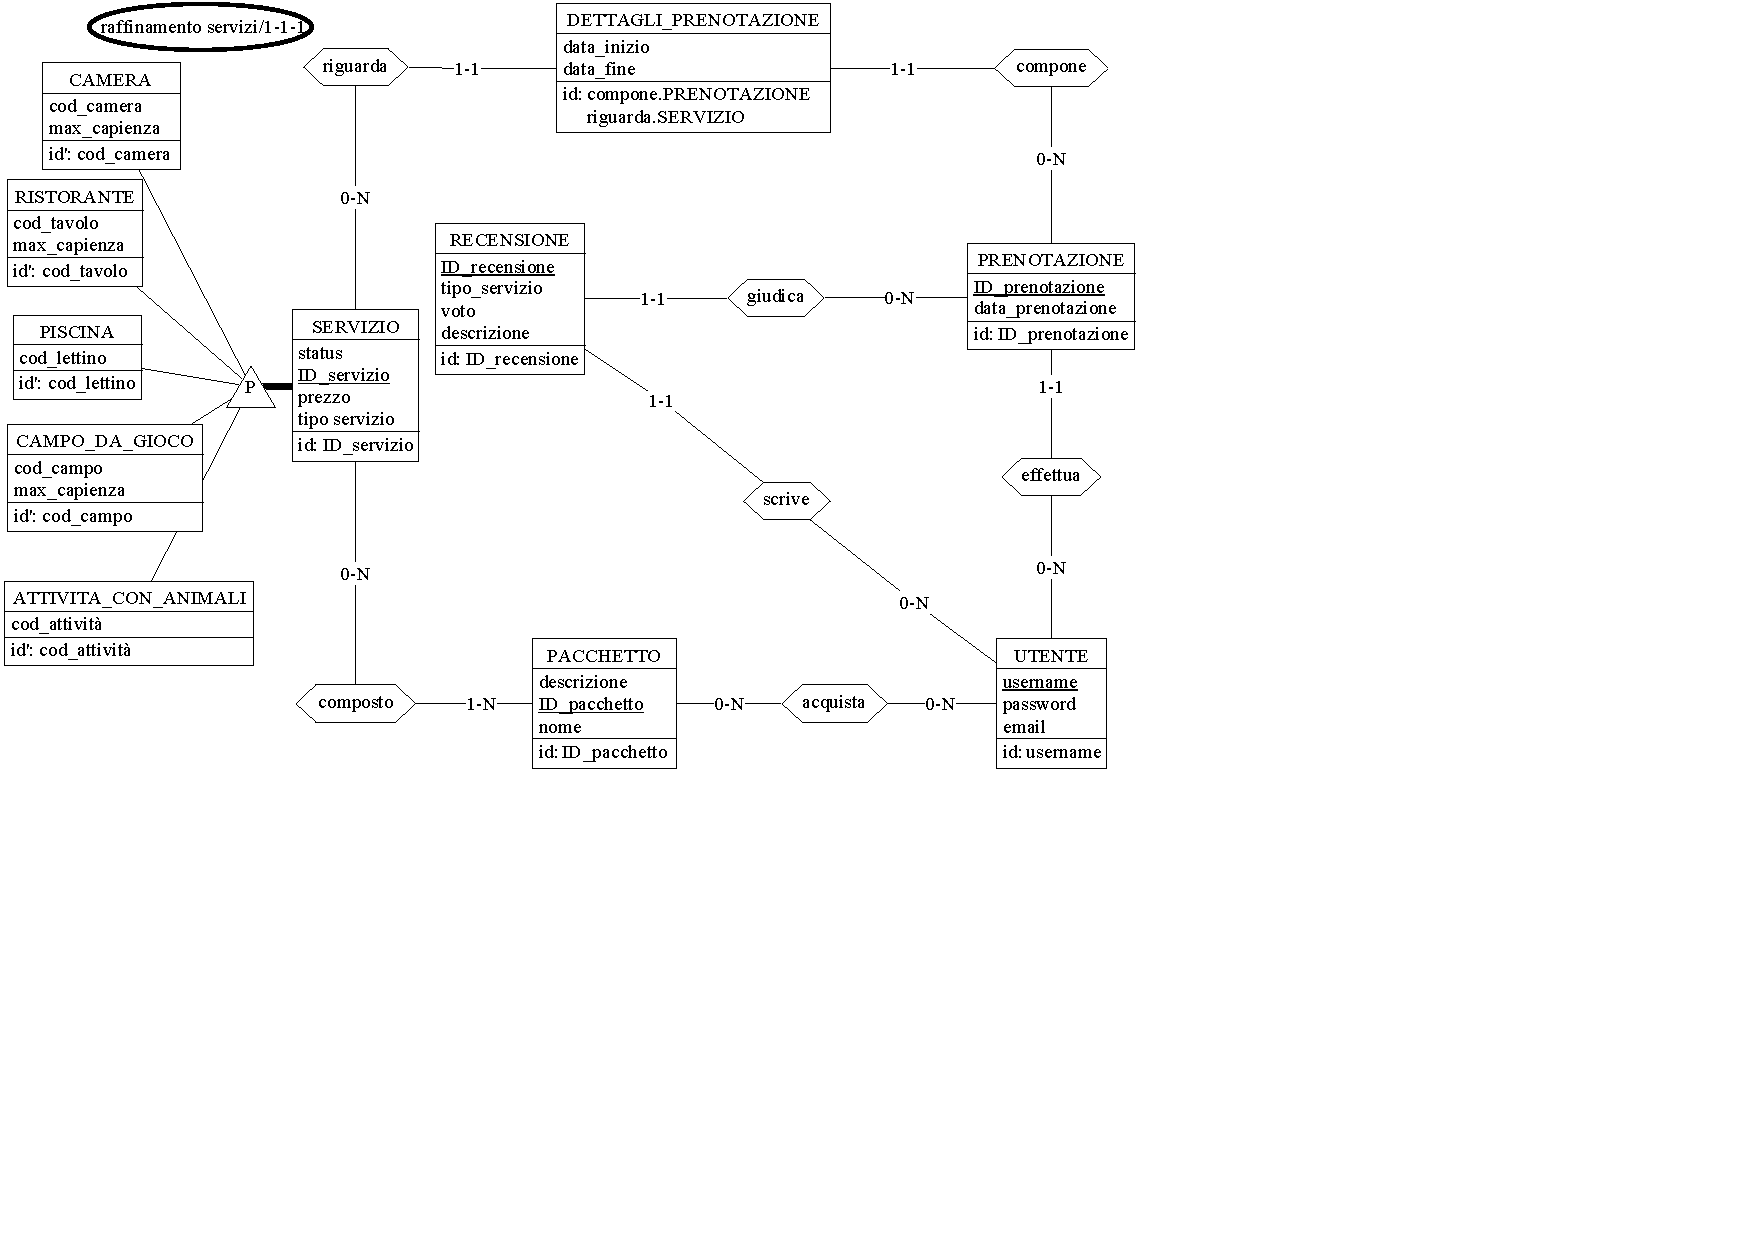
\includegraphics[width=\textwidth, trim=0 200pt 175pt 0, clip]{./pdf/raffinamento servizi.pdf}
	\caption{Schema ER, raffinamento servizi}
	\label{fig:raffinamento-servizi}
\end{figure}

\newpage
\subsection{Prodotti e ordini}
Nel modello concettuale iniziale, la gestione degli ordini e dei prodotti risultava poco dettagliata: un ordine era
semplicemente collegato a uno o più prodotti, senza possibilità di specificare informazioni aggiuntive come quantità o
prezzo unitario.

\vspace{\baselineskip}
Con il raffinamento, è stata introdotta l'entità \textbf{Dettaglio Ordine}, che funge da associazione tra \textbf{Ordine}
e \textbf{Prodotto}. Ogni dettaglio ordine consente di memorizzare, per ciascun prodotto incluso in un ordine, la quantità
acquistata e il prezzo applicato. Questo permette di rappresentare in modo accurato scenari reali come ordini
multiprodotto, applicazione di sconti o variazioni di prezzo nel tempo.

\vspace{\baselineskip}
Inoltre, viene mantenuta la generalizzazione tra \textbf{Persona} e \textbf{Utente}, già introdotta nei raffinamenti
precedenti, per distinguere i dati anagrafici comuni da quelli specifici per l'accesso al sistema e la gestione degli
ordini. Questo approccio migliora la flessibilità e la chiarezza del modello, consentendo una gestione più efficace
delle informazioni relative agli acquisti.

\begin{figure}[H]
	\centering
	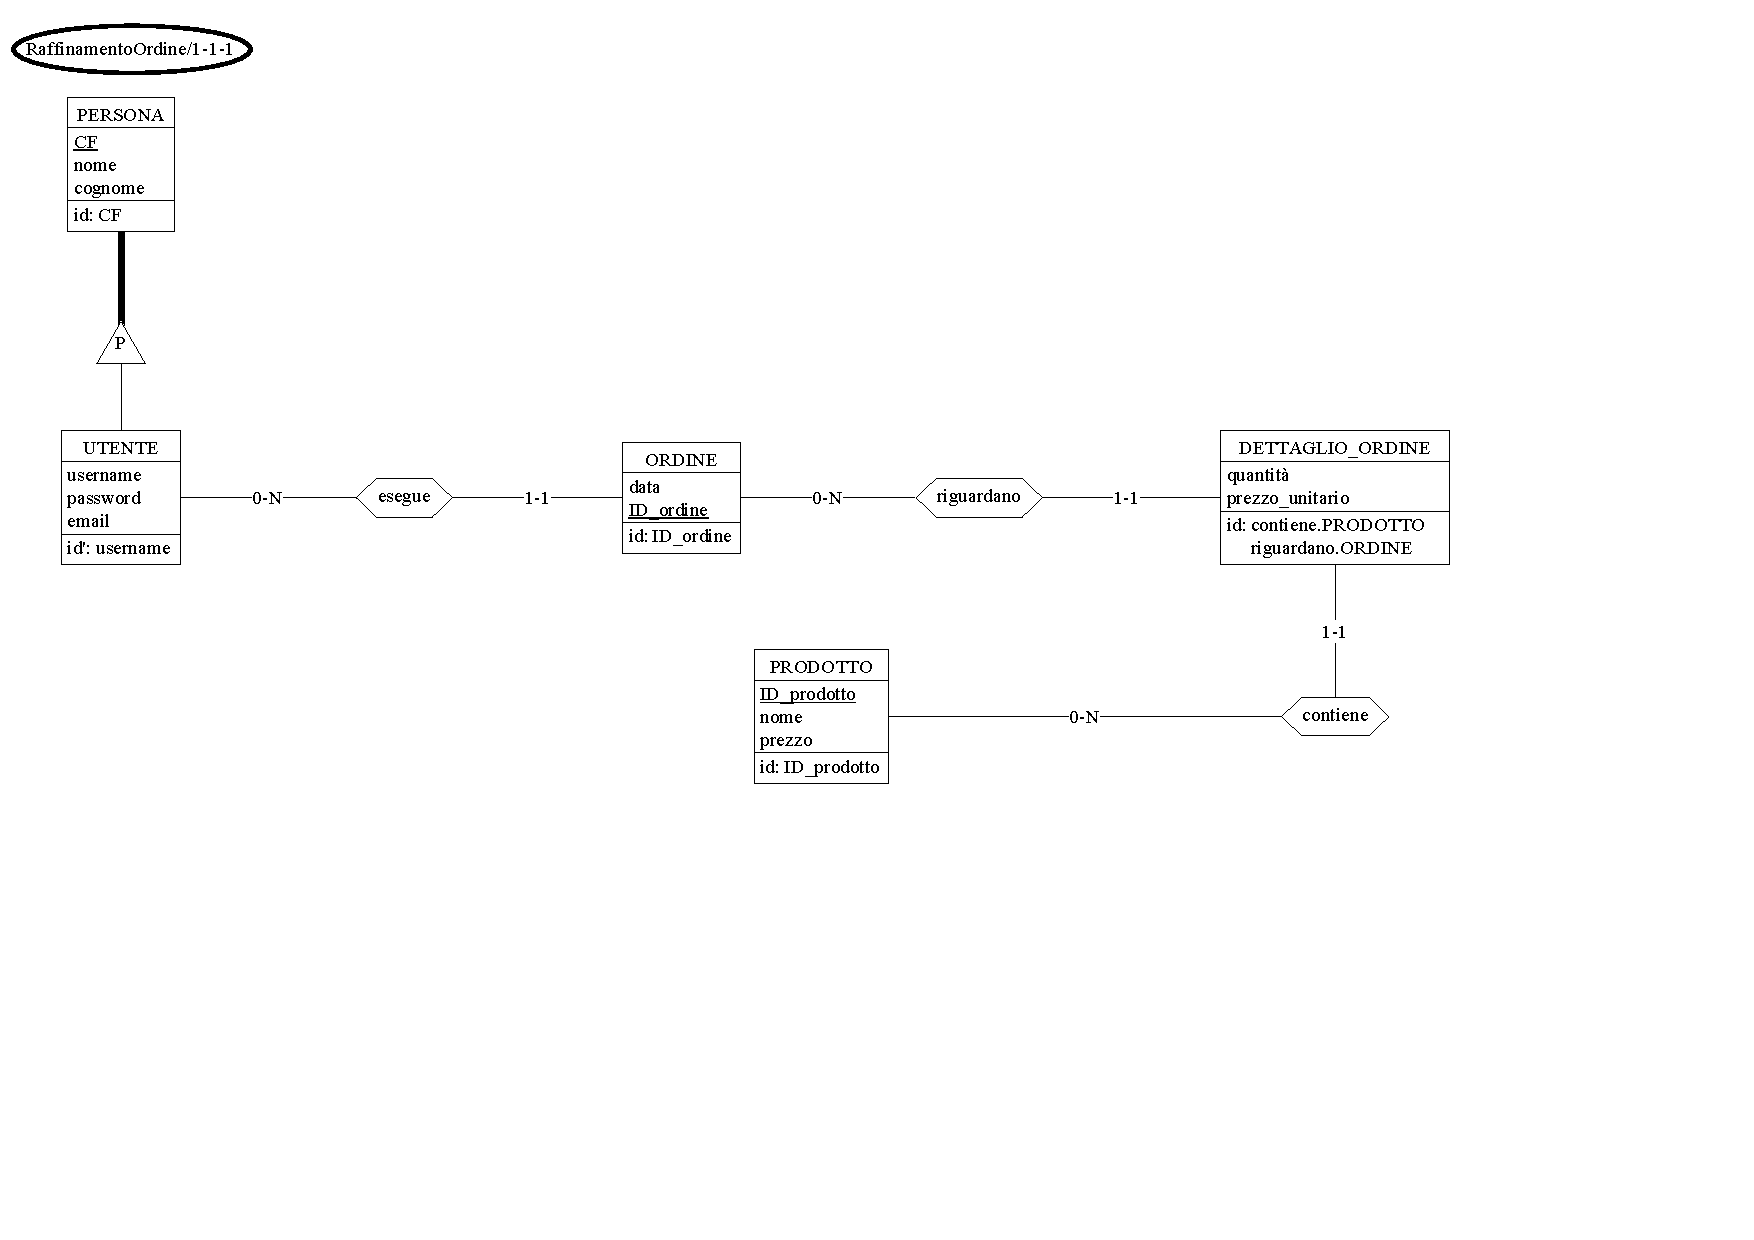
\includegraphics[width=\textwidth, trim=0 200pt 125pt 0, clip]{./pdf/raffinamento prodotto.pdf}
	\caption{Schema ER, raffinamento prodotto}
	\label{fig:raffinamento-prodotto}
\end{figure}

\newpage
\section{Schema concettuale finale}
Qui di seguito, è presente lo schema concettuale finale con tutti i raffinamenti.

\begin{figure}[H]
	\centering
	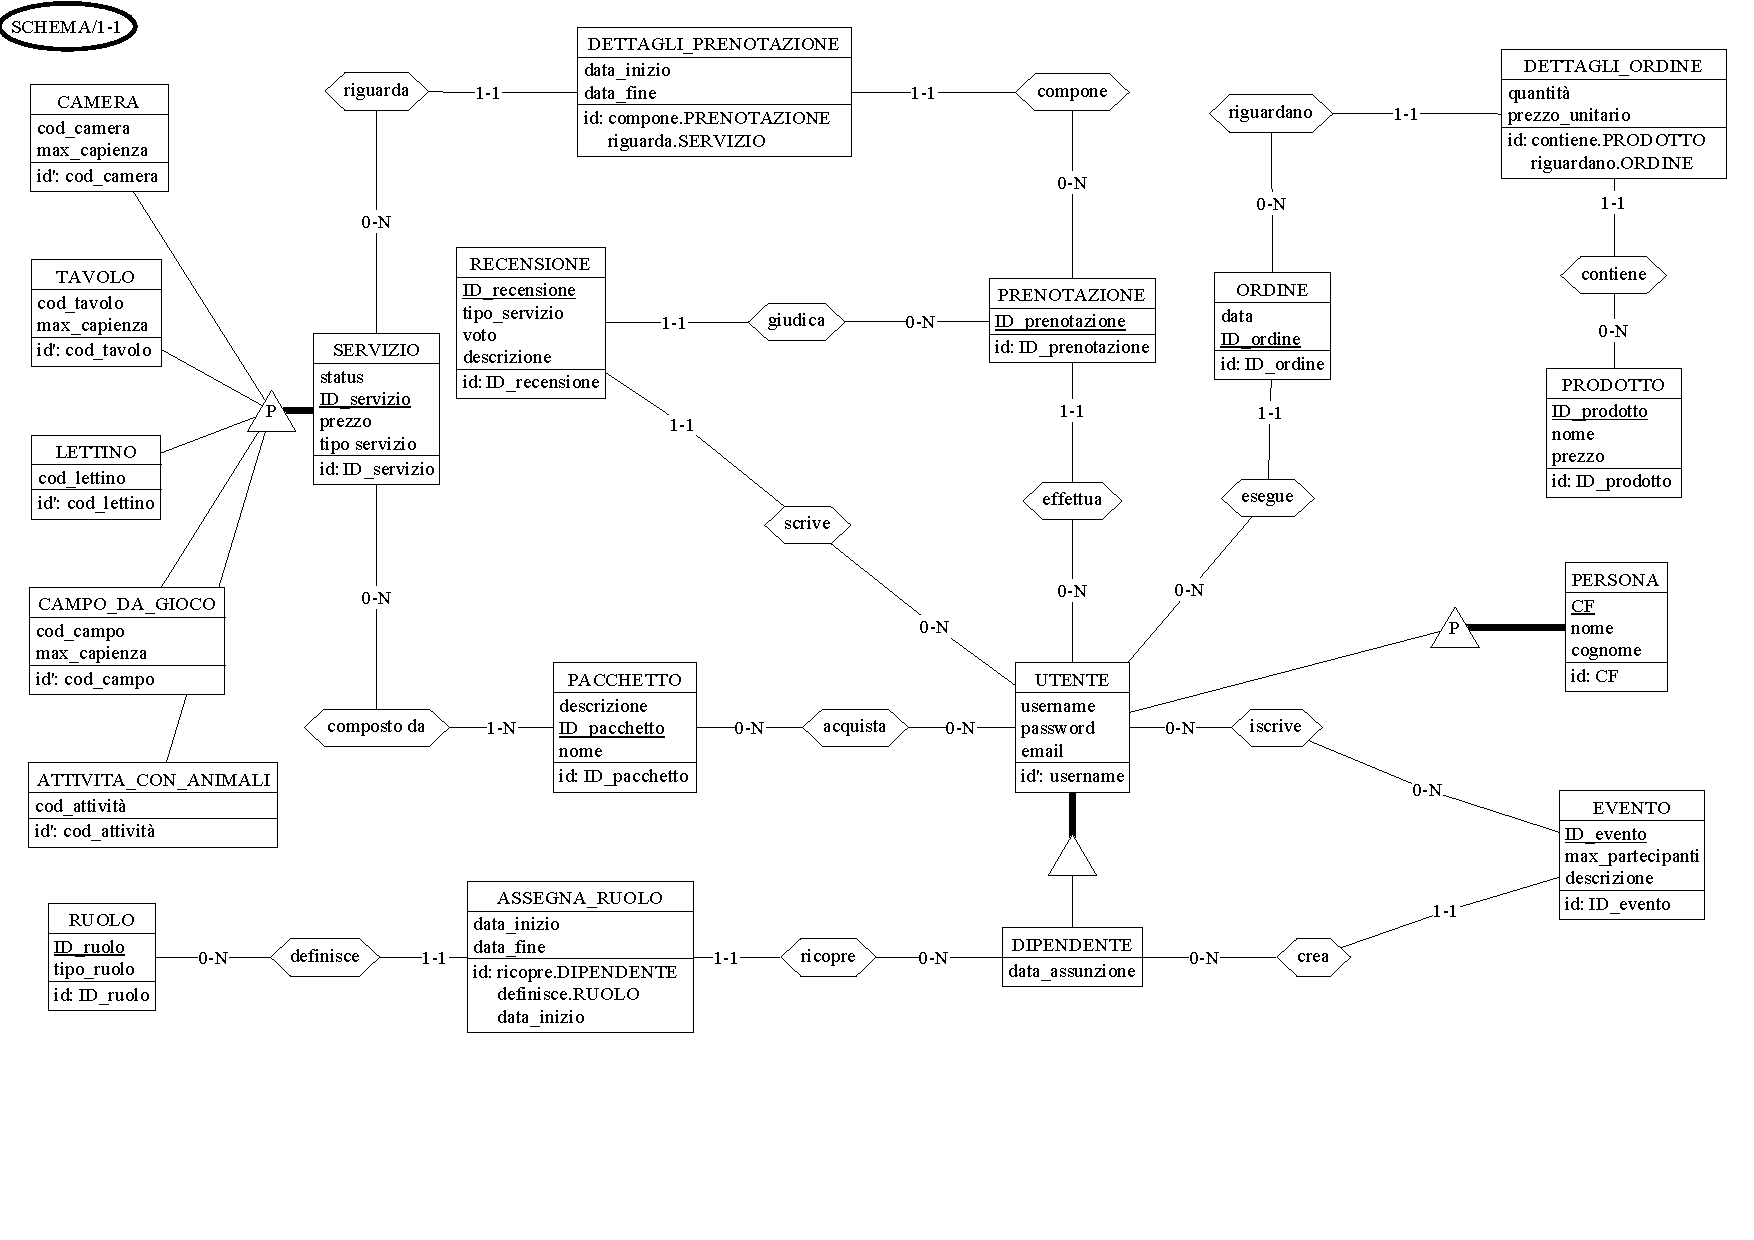
\includegraphics[width=\textwidth, trim=0 75pt 20pt 0, clip, angle=0]{./pdf/finale.pdf}
	\caption{Schema ER, schema concettuale finale}
	\label{fig:schema-finale}
\end{figure}
\newpage

\chapter{Progettazione logica}
\section{Stima del volume dei dati}
Per poter effettuare una corretta progettazione del database, è stata realizzata una stima della quantità di dati che il sistema dovrà gestire.
La stima è stata calcolata considerando un agriturismo di medie dimensioni, dotato di circa 20 camere, un ristorante e diverse attività all'aperto.
A supporto delle analisi gestionali, si è scelto di mantenere uno storico dei dati con orizzante termporale pari a un anno.
Nella tabella seguente vengono riportati i volumi stimati per entità e associazioni.
\begin{table}[H]
	\centering
	\small
	\renewcommand{\arraystretch}{1.15}
	\begin{tabularx}{\textwidth}{|X|c|c|}
		\hline
		\rowcolor{gray!20}
		\textbf{Tabella}      & \textbf{VOLUME STIMATO} & \textbf{E/A} \\
		\hline
		PERSONA               & 4500                    & E            \\
		UTENTE                & 2500                    & E            \\
		DIPENDENTE            & 25                      & E            \\
		RUOLO                 & 5                       & E            \\
		PACCHETTO             & 30                      & E            \\
		SERVIZIO              & 200                     & E            \\
		CAMERA                & 20                      & E            \\
		TAVOLO                & 100                     & E            \\
		CAMPO DA GIOCO        & 2                       & E            \\
		LETTINO               & 45                      & E            \\
		ATTIVITÀ CON ANIMALI  & 3                       & E            \\
		PRENOTAZIONE          & 2000                    & E            \\
		RECENSIONE            & 570                     & E            \\
		ORDINE                & 5000                    & E            \\
		PRODOTTO              & 150                     & E            \\
		EVENTO                & 25                      & E            \\
		ASSEGNA RUOLO         & 30                      & A            \\
		COMPOSTO DA           & 90                      & A            \\
		ACQUISTA              & 160                     & A            \\
		DETTAGLI PRENOTAZIONE & 4000                    & A            \\
		DETTAGLI ORDINE       & 15000                   & A            \\
		ISCRIVE               & 500                     & A            \\
		\hline
	\end{tabularx}
	\caption{Stima del volume dei dati}
\end{table}

\section{Descrizione operazioni}
In questa sezione vengono riportate le principali operazioni che saranno svolte sulla base di dati.
Si è stimata la frequenza con cui ogni operazione viene eseguita in media, nell'arco di una settimana,
specificando anche il tipo di utente che la effettua e il tipo di accesso al DB (letture/scritture).

\begin{table}[H]
	\centering
	\small
	\renewcommand{\arraystretch}{1.12}
	\begin{tabularx}{\textwidth}{|c|>{\raggedright\arraybackslash}X|c|c|}
		\hline
		\rowcolor{gray!20}
		\textbf{\#} & \textbf{Operazione}                                                    & \textbf{Op / 7gg} & \textbf{Tipo Utente}   \\
		\hline
		1           & \hyperref[op1]{Registrazione nuovo utente}                             & 10                & Cliente                \\
		\hline
		2           & \hyperref[op2]{Autenticazione / login}                                 & 350               & Tutti (Clienti, Staff) \\
		\hline
		3           & \hyperref[op3]{Prenotazione servizio}                                  & 125               & Cliente / Reception    \\
		\hline
		4           & \hyperref[op4]{Modifica / cancellazione prenotazione}                  & 30                & Cliente / Reception    \\
		\hline
		5           & \hyperref[op5]{Creazione / modifica pacchetto}                         & 3                 & Staff / Admin          \\
		\hline
		6           & \hyperref[op6]{Acquisto pacchetto}                                     & 15                & Cliente                \\
		\hline
		7           & \hyperref[op7]{Inserimento recensione}                                 & 40                & Cliente                \\
		\hline
		8           & \hyperref[op8]{Gestione inventario / prodotti}                         & 10                & Staff                  \\
		\hline
		9           & \hyperref[op9]{Creazione evento}                                       & 1                 & Staff / Admin          \\
		\hline
		10          & \hyperref[op10]{Iscrizione evento}                                     & 15                & Cliente                \\
		\hline
		11          & \hyperref[op11]{Creazione ordine}                                      & 25                & Cliente / Staff        \\
		\hline
		12          & \hyperref[op12]{Assegnazione / modifica ruolo dipendenti}              & 1                 & Admin                  \\
		\hline
		13          & \hyperref[op13]{Check-in / Check-out (arrivi/partenze)}                & 50                & Reception              \\
		\hline
		14          & \hyperref[op14]{Aggiornamento stato servizio (pulizia, manut.)}        & 30                & Staff operativo        \\
		\hline
		15          & \hyperref[op15]{Controllo disponibilità servizi (ricerca/filtri)}      & 550               & Tutti                  \\
		\hline
		16          & \hyperref[op16]{Generazione report settimanali (occupazione, ricavi)}  & 1                 & Admin                  \\
		\hline
		17          & \hyperref[op17]{Applicazione sconto/promozione su prenotazione/ordine} & 5                 & Staff / Admin          \\
		\hline
		18          & \hyperref[op18]{Pianificazione turni / assegnazione orari dipendenti}  & 3                 & Admin                  \\
		\hline
		19          & \hyperref[op19]{Calcolo tasso di occupazione camere mensile}           & 1                 & Admin                  \\
		\hline
		20          & \hyperref[op20]{Analisi fasce orarie più richieste per i lettini}      & 1                 & Admin / Staff          \\
		\hline
		21          & \hyperref[op21]{Individuazione pacchetto più richiesto}                & 1                 & Admin                  \\
		\hline
		22          & \hyperref[op22]{Calcolo fatturato mensile per servizio}                & 1                 & Admin                  \\
		\hline
		23          & \hyperref[op23]{Analisi servizi più inclusi nei pacchetti}             & 1                 & Admin                  \\
		\hline
	\end{tabularx}
	\caption{Numero stimato di operazioni per settimana, con tipo di utente che le effettua}
	\label{tab:operazioni-settimanali}
\end{table}

\newpage
\section{Analisi delle operazioni}
Di seguito viene riportata un'analisi per alcune delle operazioni principali sul database dell'agriturismo.
Per stimare il carico delle operazioni sul database si è deciso di introdurre i seguenti parametri:
\begin{itemize}
	\item $A_{lett}$ = numero di accessi in lettura effettuati durante l'operazione. (\textit{read})
	\item $A_{scr}$ = numero di accessi in scrittura effettuati durante l'operazione. (\textit{write})
	\item $Op_{set}$ = numero medio di volte in cui l'operazione viene eseguita in una settimana (dalla Tabella \ref{tab:operazioni-settimanali}).
\end{itemize}

\begin{enumerate}
	\item {\large \textbf{Registrazione nuovo utente}} \label{op1}

	      In questa operazione viene gestita la creazione di un nuovo utente del sistema.

	      \begin{table}[H]
		      \centering
		      \small
		      \renewcommand{\arraystretch}{1.15}
		      \begin{tabularx}{0.8\textwidth}{|X|c|c|c|}
			      \hline
			      \rowcolor{gray!20}
			      \textbf{Nome} & \textbf{Tipo} & \textbf{Numero accessi} & \textbf{S/L} \\
			      \hline
			      UTENTE        & E             & 1                       & L            \\
			      \hline
			      PERSONA       & E             & 1                       & S            \\
			      \hline
			      UTENTE        & E             & 1                       & S            \\
			      \hline
		      \end{tabularx}
	      \end{table}

	      Il flusso dunque si articola in tre parti principali:
	      \begin{enumerate}
		      \item Verificare che l'\texttt{username} ed l'\texttt{email} non siano già presenti in \texttt{UTENTE}, al fine di evitare quindi duplicati.
		      \item Inserimento dei dati anagrafici della nuova persona in \texttt{PERSONA}.
		      \item Creazione dell'utente vero e proprio in \texttt{UTENTE}, collegato alla relativa persona.
	      \end{enumerate}

	      Sono dunque presenti $A_{lettura}=1$ e $A_{scrittura}=2$.

	      Pertanto il \textbf{costo settimanale} è dato da:
	      \begin{align*}
		      C_{tot} & = O_{settimana} \cdot (A_{lett} + 2 \cdot A_{scr}) \\
		              & = 10 \cdot (1 + 2 \cdot 2)                         \\
		              & = 10 \cdot 5 = \mathbf{50}
	      \end{align*}


	\item {\large \textbf{Autenticazione / login}} \label{op2}

	      $$
		      {Op}_{sett} = 350
	      $$

	      \begin{table}[H]
		      \centering
		      \small
		      \renewcommand{\arraystretch}{1.15}
		      \begin{tabularx}{0.8\textwidth}{|X|c|c|c|}
			      \hline
			      \rowcolor{gray!20}
			      \textbf{Nome} & \textbf{Tipo} & \textbf{Numero accessi} & \textbf{S/L} \\
			      \hline
			      UTENTE        & E             & 1                       & L            \\
			      \hline
		      \end{tabularx}
	      \end{table}

	      Quindi si ha una sola operazione di lettura.
	      Pertanto $C_{tot} = 350 \cdot 1 = \mathbf{350}$

	\item {\large \textbf{Prenotazione servizio}} \label{op3}
	      $$
		      {Op}_{sett}=125
	      $$
	      In media ogni prenotazione è associata a $2$ servizi,
	      pertanto per ogni operazione di prenotazione si accede a $2$ record in \texttt{SERVIZIO}
	      e si scrivono $2$ record in \texttt{DETTAGLI\_PRENOTAZIONE}.

	      \begin{table}[H]
		      \centering
		      \small
		      \renewcommand{\arraystretch}{1.15}
		      \begin{tabularx}{0.8\textwidth}{|X|c|c|c|}
			      \hline
			      \rowcolor{gray!20}
			      \textbf{Nome}          & \textbf{Tipo} & \textbf{Numero accessi} & \textbf{S/L} \\
			      \hline
			      UTENTE                 & E             & 1                       & L            \\
			      PRENOTAZIONE           & E             & 1                       & S            \\
			      SERVIZIO               & E             & 2                       & L            \\
			      DETTAGLI\_PRENOTAZIONE & E             & 2                       & S            \\
			      \hline
		      \end{tabularx}
	      \end{table}

	      Quindi in totale si hanno $A_{lett}=3$ e $A_{scr}=3$. \\
	      Pertanto il costo settimanale è:
	      $$\mathbf{C_{tot}} = 125 \cdot (3+6)=\mathbf{1125}$$



	\item {\large \textbf{Modifica / cancellazione prenotazione}} \label{op4}

	      $$
		      {Op}_{sett} = 30
	      $$
	      In media si hanno $\frac{4000}{2000}=2$ \textbf{servizi per prenotazione}.

	      \begin{table}[H]
		      \centering
		      \small
		      \renewcommand{\arraystretch}{1.15}
		      \begin{tabularx}{0.8\textwidth}{|X|c|c|c|}
			      \hline
			      \rowcolor{gray!20}
			      \textbf{Nome}          & \textbf{Tipo} & \textbf{Numero accessi} & \textbf{S/L} \\
			      \hline
			      PRENOTAZIONE           & E             & 1                       & L            \\
			      DETTAGLI\_PRENOTAZIONE & A             & 2                       & L            \\
			      PRENOTAZIONE           & E             & 1                       & S            \\
			      DETTAGLI\_PRENOTAZIONE & A             & 2                       & S            \\
			      \hline
		      \end{tabularx}
	      \end{table}

	      Quindi in totale si hanno $A_{lett}=3$ e $A_{scr}=3$, questo perché:
	      \begin{itemize}
		      \item Si accede alla tabella \texttt{PRENOTAZIONE} per trovare la prenotazione da modificare.
		      \item Si leggono i \texttt{DETTAGLI\_PRENOTAZIONE} collegati (che sono in media 2 per prenotazione).
		      \item Infine si aggiorna o si elimina la prenotazione (se viene cancellata, si devono rimuovere anche i relativi dettagli).
	      \end{itemize}

	      Pertanto, il costo settimanale è:
	      $$
		      \mathbf{C_{tot}} = 30 \cdot (3 + 2 \cdot 3) = \mathbf{270}
	      $$


	\item {\large \textbf{Creazione / modifica pacchetto} \label{op5}}

	      In questa operazione, un membro dello staff oppure un amministratore \newline
	      crea/modifica un pacchetto, ovvero un insieme di servizi offerti ad un prezzo \newline
	      promozionale.

	      $$
		      {Op}_{set}=3
	      $$

	      In media ogni pacchetto contiene $\frac{90}{30}=3$ \textbf{servizi}

	      \begin{table}[H]
		      \centering
		      \small
		      \renewcommand{\arraystretch}{1.15}
		      \begin{tabularx}{0.8\textwidth}{|X|c|c|c|}
			      \hline
			      \rowcolor{gray!20}
			      \textbf{Nome} & \textbf{Tipo} & \textbf{Numero accessi} & \textbf{S/L} \\
			      \hline
			      PACCHETTO     & E             & 1                       & S            \\
			      SERVIZIO      & E             & 3                       & L            \\
			      COMPOSTO\_DA  & A             & 3                       & L            \\
			      \hline
		      \end{tabularx}
	      \end{table}
	      Si hanno dunque $A_{lett}=3$ e $A_{scr}=4$. \\
	      Questo perché:
	      \begin{itemize}
		      \item si inserisce o aggiorna il record del \texttt{PACCHETTO};
		      \item si leggono in media 3 record di \texttt{SERVIZIO} per verificare la loro esistenza;
		      \item si scrivono in media 3 record nella relazione \texttt{COMPOSTO\_DA}, che collega i 	servizi al pacchetto.
	      \end{itemize}

	      Pertanto il costo settimanale è:
	      $$
		      C_{tot} = 3 \cdot (3 + 2 \cdot 4) = \mathbf{33}
	      $$

	\item {\large \textbf{Acquisto pacchetto}} \label{op6}

	      $$
		      {Op}_{sett} = 15
	      $$

	      In media ogni pacchetto contiene $\frac{90}{30}=3$ \textbf{servizi}.

	      \begin{table}[H]
		      \centering
		      \small
		      \renewcommand{\arraystretch}{1.15}
		      \begin{tabularx}{0.85\textwidth}{|X|c|c|c|}
			      \hline
			      \rowcolor{gray!20}
			      \textbf{Nome}          & \textbf{Tipo} & \textbf{Numero accessi} & \textbf{S/L} \\
			      \hline
			      UTENTE                 & E             & 1                       & L            \\
			      PACCHETTO              & E             & 1                       & L            \\
			      ACQUISTA               & A             & 1                       & S            \\
			      SERVIZIO               & E             & 3                       & L            \\
			      DETTAGLI\_PRENOTAZIONE & A             & 3                       & S            \\
			      \hline
		      \end{tabularx}
	      \end{table}

	      Quindi in totale si hanno $A_{lett}=5$ e $A_{scr}=4$.

	      Questo perché:
	      \begin{itemize}
		      \item si effettua in \texttt{UTENTE} una lettura per verificare chi effettua l'acquisto;
		      \item si legge il \texttt{PACCHETTO} scelto;
		      \item si scrive la relazione \texttt{ACQUISTA} per collegare utente e pacchetto;
		      \item si leggono i \texttt{SERVIZI} contenuti nel pacchetto;
		      \item si inseriscono i corrispondenti record in \texttt{DETTAGLI\_PRENOTAZIONE}.
	      \end{itemize}

	      Pertanto il costo settimanale è:
	      \[
		      \mathbf{C_{tot}} = 15 \cdot (5 + 2 \cdot 4) = \mathbf{195}
	      \]


	\item {\large \textbf{Inserimento recensione}} \label{op7}

	      $$
		      {Op}_{sett} = 40
	      $$

	      In media ogni pacchetto contiene $\frac{90}{30}=3$ \textbf{servizi}.

	      \begin{table}[H]
		      \centering
		      \small
		      \renewcommand{\arraystretch}{1.15}
		      \begin{tabularx}{0.8\textwidth}{|X|c|c|c|}
			      \hline
			      \rowcolor{gray!20}
			      \textbf{Nome} & \textbf{Tipo} & \textbf{Numero accessi} & \textbf{S/L} \\
			      \hline
			      UTENTE        & E             & 1                       & L            \\
			      SERVIZIO      & E             & 1                       & L            \\
			      RECENSIONE    & E             & 1                       & S            \\
			      \hline
		      \end{tabularx}
	      \end{table}

	      Quindi in totale si hanno $A_{lett}=2$ e $A_{scr}=1$.

	      Questo perché:
	      \begin{itemize}
		      \item si legge l'\texttt{UTENTE} che lascia la recensione;
		      \item si verifica il \texttt{SERVIZIO} a cui si riferisce;
		      \item si inserisce un record in \texttt{RECENSIONE}.
	      \end{itemize}

	      Pertanto il costo settimanale è:
	      $$\mathbf{C_{tot}} = 40 \cdot (2 + 2 \cdot 1) = \mathbf{160}$$


	\item {\large \textbf{Gestione inventario / prodotti}} \label{op8}

	      Per gestione inventario si intende l'aggiornamento dei prodotti del ristorante/bar da parte dello staff.
	      $$
		      {Op}_{sett} = 10
	      $$

	      \begin{table}[H]
		      \centering
		      \small
		      \renewcommand{\arraystretch}{1.15}
		      \begin{tabularx}{0.8\textwidth}{|X|c|c|c|}
			      \hline
			      \rowcolor{gray!20}
			      \textbf{Nome} & \textbf{Tipo} & \textbf{Numero accessi} & \textbf{S/L} \\
			      \hline
			      PRODOTTO      & E             & 1                       & L            \\
			      PRODOTTO      & E             & 1                       & S            \\
			      \hline
		      \end{tabularx}
	      \end{table}

	      Quindi in totale si hanno $A_{lett}=1$ e $A_{scr}=1$.

	      Questo perché:
	      \begin{itemize}
		      \item prima leggiamo il record del \texttt{PRODOTTO} per verificare l'esistenza di dati attuali
		      \item per poi aggiornarlo (se esiste) o inserirlo
	      \end{itemize}

	      Pertanto il costo settimanale è:
	      $$\mathbf{C_{tot}} = 10 \cdot (1 + 2 \cdot 1) = \mathbf{30}$$

	\item {\large \textbf{Creazione evento}} \label{op9}

	      $$
		      {Op}_{sett} = 1
	      $$

	      \begin{table}[H]
		      \centering
		      \small
		      \renewcommand{\arraystretch}{1.15}
		      \begin{tabularx}{0.8\textwidth}{|X|c|c|c|}
			      \hline
			      \rowcolor{gray!20}
			      \textbf{Nome} & \textbf{Tipo} & \textbf{Numero accessi} & \textbf{S/L} \\
			      \hline
			      EVENTO        & E             & 1                       & S            \\
			      \hline
		      \end{tabularx}
	      \end{table}

	      Questo perchè l'operazione comporta semplicemente l'inserimento di un \newline nuovo \texttt{EVENTO}.

	      Quindi si ha solamente un'operazione di scrittura:
	      $$
		      \mathbf{C_{tot}} = 1 \cdot (0 + 2 \cdot 1) = \mathbf{2}
	      $$

	\item {\large \textbf{Iscrizione evento}} \label{op10}

	      $$
		      {Op}_{sett} = 15
	      $$

	      In media ad un evento si iscrivono $\frac{500}{25}=20$ \textbf{iscritti}

	      \begin{table}[H]
		      \centering
		      \small
		      \renewcommand{\arraystretch}{1.15}
		      \begin{tabularx}{0.9\textwidth}{|X|c|c|c|}
			      \hline
			      \rowcolor{gray!20}
			      \textbf{Nome} & \textbf{Tipo} & \textbf{Numero accessi} & \textbf{S/L} \\
			      \hline
			      UTENTE        & E             & 1                       & L            \\
			      EVENTO        & E             & 1                       & L            \\
			      ISCRIVE       & A             & 1                       & S            \\
			      \hline
		      \end{tabularx}
	      \end{table}

	      Questo perché:
	      \begin{itemize}
		      \item si legge l'\texttt{UTENTE} che si iscrive;
		      \item si legge l'\texttt{EVENTO} scelto;
		      \item si inserisce un nuovo record nella \texttt{ISCRIVE}.
	      \end{itemize}

	      Quindi: $A_{lett}=2$, $A_{scr}=1$.
	      Pertanto il costo settimanale è:
	      $$\mathbf{C_{tot}} = 15 \cdot (2 + 2 \cdot 1) = \mathbf{60}$$


	\item {\large \textbf{Creazione Ordine}} \label{op11}

	      $$
		      {Op}_{sett} = 25
	      $$

	      In media ogni ordine contiene $\frac{15000}{5000}=3$ \textbf{prodotti}.

	      \begin{table}[H]
		      \centering
		      \small
		      \renewcommand{\arraystretch}{1.15}
		      \begin{tabularx}{0.9\textwidth}{|X|c|c|c|}
			      \hline
			      \rowcolor{gray!20}
			      \textbf{Nome}    & \textbf{Tipo} & \textbf{Numero accessi} & \textbf{S/L} \\
			      \hline
			      UTENTE           & E             & 1                       & L            \\
			      ORDINE           & E             & 1                       & S            \\
			      PRODOTTO         & E             & 3                       & L            \\
			      DETTAGLI\_ORDINE & A             & 3                       & S            \\
			      \hline
		      \end{tabularx}
	      \end{table}

	      Questo perché:
	      \begin{itemize}
		      \item si legge l'\texttt{UTENTE} che effettua l'ordine;
		      \item si inserisce un nuovo record in \texttt{ORDINE};
		      \item si leggono in media 3 \texttt{PRODOTTI};
		      \item e si scrivono 3 record in \texttt{DETTAGLI\_ORDINE}.
	      \end{itemize}

	      Quindi: $A_{lett}=4$, $A_{scr}=4$.
	      Pertanto il costo settimanale è:
	      $$\mathbf{C_{tot}} = 25 \cdot (4 + 2 \cdot 4) = \mathbf{300}$$



	\item {\large \textbf{Assegnazione / modifica ruolo dipendenti}} \label{op12}
	      $$
		      Op_{sett} = 1
	      $$

	      \begin{table}[H]
		      \centering
		      \small
		      \renewcommand{\arraystretch}{1.15}
		      \begin{tabularx}{0.8\textwidth}{|X|c|c|c|}
			      \hline
			      \rowcolor{gray!20}
			      \textbf{Nome}  & \textbf{Tipo} & \textbf{Numero accessi} & \textbf{S/L} \\
			      \hline
			      DIPENDENTE     & E             & 1                       & L            \\
			      RUOLO          & E             & 1                       & L            \\
			      ASSEGNA\_RUOLO & A             & 1                       & S            \\
			      \hline
		      \end{tabularx}
	      \end{table}

	      In questa operazione si assegna o modifica il ruolo di un dipendente:
	      \begin{itemize}
		      \item Si legge il \texttt{DIPENDENTE}.
		      \item Si legge il \texttt{RUOLO}.
		      \item Si inserisce/aggiorna l'associazione in \texttt{ASSEGNA\_RUOLO}.
	      \end{itemize}

	      Totale: $A_{lett}=2$, $A_{scr}=1$.
	      \[
		      C_{tot} = 1 \cdot (2 + 2 \cdot 1) = \mathbf{4}
	      \]


	\item {\large \textbf{Check-in / Check-out}} \label{op13}

	      Questa operazione gestisce l'arrivo o la partenza di un cliente.
	      $$
		      Op_{sett} = 50
	      $$


	      \begin{table}[H]
		      \centering
		      \small
		      \renewcommand{\arraystretch}{1.15}
		      \begin{tabularx}{0.8\textwidth}{|X|c|c|c|}
			      \hline
			      \rowcolor{gray!20}
			      \textbf{Nome}          & \textbf{Tipo} & \textbf{Numero accessi} & \textbf{S/L} \\
			      \hline
			      PRENOTAZIONE           & E             & 1                       & L            \\
			      DETTAGLI\_PRENOTAZIONE & A             & 2                       & L            \\
			      DETTAGLI\_PRENOTAZIONE & A             & 2                       & S            \\
			      \hline
		      \end{tabularx}
	      \end{table}

	      \begin{itemize}
		      \item Si legge la \texttt{PRENOTAZIONE}.
		      \item Si leggono i \texttt{DETTAGLI\_PRENOTAZIONE} collegati (in media ci sono 2).
		      \item Si aggiornano gli stessi dettagli con lo stato di check-in/check-out.
	      \end{itemize}

	      Quindi ci sono $A_{lett}=3$ e $A_{scr}=2$. \\
	      Pertanto il costo settimanale è dato da:
	      $$
		      \mathbf{C_{tot}} = 50 \cdot (3 + 2 \cdot 2) = \mathbf{350}
	      $$

	\item {\large \textbf{Aggiornamento stato servizio}} \label{op14}

	      Questa operazione spiega quante volte lo staff aggiorna lo stato di un servizio.
	      $$
		      Op_{sett} = 30
	      $$

	      \begin{table}[H]
		      \centering
		      \small
		      \renewcommand{\arraystretch}{1.15}
		      \begin{tabularx}{0.8\textwidth}{|X|c|c|c|}
			      \hline
			      \rowcolor{gray!20}
			      \textbf{Nome} & \textbf{Tipo} & \textbf{Numero accessi} & \textbf{S/L} \\
			      \hline
			      SERVIZIO      & E             & 1                       & L            \\
			      SERVIZIO      & E             & 1                       & S            \\
			      \hline
		      \end{tabularx}
	      \end{table}

	      \begin{itemize}
		      \item Si legge il \texttt{SERVIZIO}.
		      \item Si aggiorna lo stato (es. disponibile, in manutenzione, occupato).
	      \end{itemize}

	      Quindi ci sono $A_{lett}=1$ e $A_{scr}=1$.
	      $$\mathbf{C_{tot}} = 30 \cdot (1 + 2 \cdot 1) = \mathbf{90}$$

	\item {\large \textbf{Controllo disponibilità servizi}} \label{op15}

	      Un utente o lo staff verificano la disponibilità di un servizio in un dato periodo.
	      Si assume che gli utenti guardino in media 3 servizi e che, quindi, non consultino solamente uno.

	      $$
		      Op_{sett} = 550
	      $$

	      \begin{table}[H]
		      \centering
		      \small
		      \renewcommand{\arraystretch}{1.15}
		      \begin{tabularx}{0.8\textwidth}{|X|c|c|c|}
			      \hline
			      \rowcolor{gray!20}
			      \textbf{Nome} & \textbf{Tipo} & \textbf{Numero accessi} & \textbf{S/L} \\
			      \hline
			      SERVIZIO      & E             & 3                       & L            \\
			      \hline
		      \end{tabularx}
	      \end{table}

	      \begin{itemize}
		      \item Gli utenti ricercano tra più \texttt{SERVIZI} (camere, tavoli, attività, ecc.).
		      \item Operazione di sola lettura.
	      \end{itemize}

	      Quindi solamente $A_{lett}=3$.

	      $$\mathbf{C_{tot}} = 550 \cdot 3 = \mathbf{1650}$$

	\item {\large \textbf{Generazione report settimanali}} \label{op16}

	      Lo staff genera report riassuntivi sulle prenotazioni e sugli ordini.
	      In media un report include 20 prenotazioni e 10 ordini.
	      $$
		      Op_{sett} = 1
	      $$

	      \begin{table}[H]
		      \centering
		      \small
		      \renewcommand{\arraystretch}{1.15}
		      \begin{tabularx}{0.8\textwidth}{|X|c|c|c|}
			      \hline
			      \rowcolor{gray!20}
			      \textbf{Nome} & \textbf{Tipo} & \textbf{Numero accessi} & \textbf{S/L} \\
			      \hline
			      PRENOTAZIONE  & E             & 20                      & L            \\
			      ORDINE        & E             & 10                      & L            \\
			      \hline
		      \end{tabularx}
	      \end{table}

	      \begin{itemize}
		      \item L'admin richiede statistiche (occupazione, ricavi).
		      \item Molte letture, nessuna scrittura.
	      \end{itemize}

	      L'operazione è di sola lettura perché consiste nell'estrarre dati da più entità per creare il report.
	      $$\mathbf{C_{tot}} = 1 \cdot (30) = \mathbf{30}$$


	\item {\large \textbf{Applicazione sconto / promozione}} \label{op17}
	      Un amministratore o un membro dello staff inserisce o modifica una promozione su pacchetti o servizi.
	      $$
		      Op_{sett} = 5
	      $$

	      \begin{table}[H]
		      \centering
		      \small
		      \renewcommand{\arraystretch}{1.15}
		      \begin{tabularx}{0.8\textwidth}{|X|c|c|c|}
			      \hline
			      \rowcolor{gray!20}
			      \textbf{Nome}         & \textbf{Tipo} & \textbf{Numero accessi} & \textbf{S/L} \\
			      \hline
			      PRENOTAZIONE / ORDINE & E             & 1                       & L            \\
			      PRENOTAZIONE / ORDINE & E             & 1                       & S            \\
			      \hline
		      \end{tabularx}
	      \end{table}

	      \begin{itemize}
		      \item Si legge la prenotazione o l'ordine.
		      \item Si aggiorna applicando sconto o promozione.
	      \end{itemize}

	      Quindi si ha $A_{lett}=1$ e $A_{scr}=1$.
	      $$\mathbf{C_{tot}} = 5 \cdot (1 + 2 \cdot 1) = \mathbf{15}$$

	\item {\large \textbf{Pianificazione turni / orari dipendenti}} \label{op18}
	      $$
		      Op_{sett} = 3
	      $$

	      \begin{table}[H]
		      \centering
		      \small
		      \renewcommand{\arraystretch}{1.15}
		      \begin{tabularx}{0.8\textwidth}{|X|c|c|c|}
			      \hline
			      \rowcolor{gray!20}
			      \textbf{Nome} & \textbf{Tipo} & \textbf{Numero accessi} & \textbf{S/L} \\
			      \hline
			      DIPENDENTE    & E             & 1                       & L            \\
			      ORARIO\_TURNO & A             & 1                       & S            \\
			      \hline
		      \end{tabularx}
	      \end{table}

	      \begin{itemize}
		      \item Si leggono i dipendenti.
		      \item Si inserisce/aggiorna la pianificazione in \texttt{ORARIO\_TURNO}.
	      \end{itemize}

	      Totale: $A_{lett}=1$, $A_{scr}=1$.
	      $$C_{tot} = 3 \cdot (1 + 2 \cdot 1) = \mathbf{9}$$


	\item {\large \textbf{Calcolo tasso di occupazione camere mensile}} \label{op19}
	      $$
		      {Op}_{sett} = 1
	      $$
	      È un'operazione gestionale volta ad individuare i mesi/scenari a bassa occupazione e pianificare promozioni mirate.

	      \begin{table}[H]
		      \centering
		      \small
		      \renewcommand{\arraystretch}{1.15}
		      \begin{tabularx}{0.8\textwidth}{|X|c|c|c|}
			      \hline
			      \rowcolor{gray!20}
			      \textbf{Nome}          & \textbf{Tipo} & \textbf{Numero accessi} & \textbf{S/L} \\
			      \hline
			      PRENOTAZIONE           & E             & 2000                    & L            \\
			      DETTAGLI\_PRENOTAZIONE & A             & 4000                    & L            \\
			      CAMERA                 & E             & 20                      & L            \\
			      SERVIZIO               & E             & 200                     & L            \\
			      UTENTE                 & E             & 2000                    & L            \\
			      \hline
		      \end{tabularx}
	      \end{table}

	      Questo perché:
	      \begin{itemize}
		      \item si leggono tutte le \texttt{PRENOTAZIONI} effettuate,
		      \item si consultano i \texttt{DETTAGLI\_PRENOTAZIONE} per sapere quali camere sono state usate,
		      \item si leggono le entità \texttt{CAMERA} e \texttt{SERVIZIO} per filtrare i soli servizi di tipo “camera”,
		      \item si accede agli \texttt{UTENTI} collegati per fini di reportistica (segmentazione per tipologia di cliente).
	      \end{itemize}

	      Si hanno quindi: $A_{\text{lett}} = 2000 + 4000 + 20 + 200 + 2000 = 8220$
	      Pertanto il costo settimanale è dato da:
	      $$
		      \mathbf{C_{tot}} = 1 \cdot (8220 + 0) = \mathbf{8220}
	      $$


	\item {\large \textbf{Analisi fasce orarie più richieste per i lettini}} \label{op20}

	      È un'operazione volta a dimensionare i turni del personale sui picchi di domanda, al fine di migliorare il servizio e gestire al meglio le risorse.

	      \begin{table}[H]
		      \centering
		      \small
		      \renewcommand{\arraystretch}{1.15}
		      \begin{tabularx}{0.8\textwidth}{|X|c|c|c|}
			      \hline
			      \rowcolor{gray!20}
			      \textbf{Nome}          & \textbf{Tipo} & \textbf{Numero accessi} & \textbf{S/L} \\
			      \hline
			      DETTAGLI\_PRENOTAZIONE & A             & 4000                    & L            \\
			      LETTINO                & E             & 45                      & L            \\
			      PRENOTAZIONE           & E             & 2000                    & L            \\
			      UTENTE                 & E             & 2000                    & L            \\
			      \hline
		      \end{tabularx}
	      \end{table}

	      Questo perché:
	      \begin{itemize}
		      \item i \texttt{DETTAGLI\_PRENOTAZIONE} permettono di risalire a quali lettini sono stati richiesti e quando,
		      \item la tabella \texttt{LETTINO} serve a distinguere i diversi lettini,
		      \item da \texttt{PRENOTAZIONE} si ricavano le date/ore di utilizzo,
		      \item si leggono gli \texttt{UTENTI} per distinguere tipologie di clientela (es. ospiti giornalieri vs soggiornanti).
	      \end{itemize}

	      Si ha quindi $A_{\text{lett}} = 4000 + 45 + 2000 + 2000 = 8045$
	      $$\mathbf{C_{tot}} = 1 \cdot (8045 + 0) = \mathbf{8045}$$


	\item {\large \textbf{Individuazione pacchetto più richiesto}} \label{op21}
	      $$
		      {Op}_{sett} = 1
	      $$
	      Per promuovere l'esperienza più popolare e migliorare i servizi collegati.

	      \begin{table}[H]
		      \centering
		      \small
		      \renewcommand{\arraystretch}{1.15}
		      \begin{tabularx}{0.8\textwidth}{|X|c|c|c|}
			      \hline
			      \rowcolor{gray!20}
			      \textbf{Nome} & \textbf{Tipo} & \textbf{Numero accessi} & \textbf{S/L} \\
			      \hline
			      ACQUISTA      & A             & 160                     & L            \\
			      PACCHETTO     & E             & 30                      & L            \\
			      UTENTE        & E             & 160                     & L            \\
			      COMPOSTO\_DA  & A             & 90                      & L            \\
			      SERVIZIO      & E             & 200                     & L            \\
			      \hline
		      \end{tabularx}
	      \end{table}

	      Questo perché:
	      \begin{itemize}
		      \item si leggono le relazioni \texttt{ACQUISTA} per sapere quanti pacchetti sono stati acquistati,
		      \item da \texttt{PACCHETTO} si individuano i pacchetti specifici,
		      \item gli \texttt{UTENTI} permettono di segmentare la clientela,
		      \item da \texttt{COMPOSTO\_DA} e \texttt{SERVIZIO} si vedono i contenuti del pacchetto più richiesto.
	      \end{itemize}

	      Si ha $A_{\text{lett}} = 160 + 30 + 160 + 90 + 200 = 640$
	      $$\mathbf{C_{tot}} = 1 \cdot (640 + 0) = \mathbf{640}$$


	\item {\large \textbf{Calcolo fatturato per servizio}} \label{op22}
	      $$
		      {Op}_{sett} = 1
	      $$
	      Per valutare la redditività dei singoli servizi e riallocare il budget.

	      \begin{table}[H]
		      \centering
		      \small
		      \renewcommand{\arraystretch}{1.15}
		      \begin{tabularx}{0.8\textwidth}{|X|c|c|c|}
			      \hline
			      \rowcolor{gray!20}
			      \textbf{Nome}    & \textbf{Tipo} & \textbf{Numero accessi} & \textbf{S/L} \\
			      \hline
			      ORDINE           & E             & 5000                    & L            \\
			      DETTAGLI\_ORDINE & A             & 15000                   & L            \\
			      SERVIZIO         & E             & 200                     & L            \\
			      PRODOTTO         & E             & 500                     & L            \\
			      UTENTE           & E             & 5000                    & L            \\
			      \hline
		      \end{tabularx}
	      \end{table}

	      Questo perché:
	      \begin{itemize}
		      \item si leggono gli \texttt{ORDINI} registrati,
		      \item da \texttt{DETTAGLI\_ORDINE} si ottiene la quantità/prezzo dei prodotti acquistati,
		      \item da \texttt{SERVIZIO} si mappa l'ordine a uno specifico servizio (es. ristorante, spa),
		      \item i \texttt{PRODOTTI} collegati aiutano a distinguere la parte di ricavi da beni materiali,
		      \item gli \texttt{UTENTI} permettono di segmentare la clientela in termini di spesa.
	      \end{itemize}

	      Si hanno quindi $A_{\text{lett}} = 5000 + 15000 + 200 + 500 + 5000 = 25700$
	      $$\mathbf{C_{tot}} = 1 \cdot (25700 + 0) = \mathbf{25700}$$


	\item {\large \textbf{Analisi servizi più inclusi nei pacchetti}} \label{op23}
	      $$
		      {Op}_{sett} = 1
	      $$
	      Questa operazione è necessaria a capire le combinazioni preferite e progettare nuovi pacchetti garantendo i servizi più richiesti.

	      \begin{table}[H]
		      \centering
		      \small
		      \renewcommand{\arraystretch}{1.15}
		      \begin{tabularx}{0.8\textwidth}{|X|c|c|c|}
			      \hline
			      \rowcolor{gray!20}
			      \textbf{Nome} & \textbf{Tipo} & \textbf{Numero accessi} & \textbf{S/L} \\
			      \hline
			      PACCHETTO     & E             & 30                      & L            \\
			      SERVIZIO      & E             & 200                     & L            \\
			      COMPOSTO\_DA  & A             & 90                      & L            \\
			      ACQUISTA      & A             & 160                     & L            \\
			      UTENTE        & E             & 160                     & L            \\
			      \hline
		      \end{tabularx}
	      \end{table}

	      Questo perché:
	      \begin{itemize}
		      \item si leggono i \texttt{PACCHETTI} definiti,
		      \item si consultano i \texttt{SERVIZI} inclusi tramite la relazione \texttt{COMPOSTO\_DA},
		      \item la relazione \texttt{ACQUISTA} mostra quali pacchetti sono effettivamente scelti,
		      \item si leggono gli \texttt{UTENTI} per analizzare preferenze della clientela.
	      \end{itemize}

	      Si ha $A_{\text{lett}} = 30 + 200 + 90 + 160 + 160 = 640$
	      $$\mathbf{C_{tot}} = 1 \cdot (640 + 0) = \mathbf{640}$$
\end{enumerate}

\section{Analisi delle ridondanze}
In questa sezione vengono analizzate le rindondaze individuate nello schema concettuale valutandone l'impatto sul
costo delle operazioni e decidendo se mantenerle o meno.

\begin{itemize}
	\item \textbf{prezzo unitario} in DETTAGLIO ORDINE
	\item \textbf{prezzo} in DETTAGLIO ORDINE
	\item \textbf{quantità} in DETTAGLI ORDINE
	\item \textbf{tipo servizio} in RECENSIONE
	\item \textbf{status} in SERVIZIO
\end{itemize}

\subsection{Analisi attributo prezzo unitario in DETTAGLI ORDINE}

\begin{table}[H]
	\centering
	\begin{tabular}{|l|c|c|}
		\hline
		\textbf{Operazione}                          & \textbf{Con ridondanza} & \textbf{Senza ridondanza} \\
		\hline
		Visualizzazione dettagli di un ordine        & 500                     & 1000                      \\
		Riepilogo storico ordini con prezzi corretti & 1000                    & 2000                      \\
		\hline
		\textbf{Totale}                              & 1500                    & 3000                      \\
		\hline
	\end{tabular}
	\caption{Analisi attributo \texttt{prezzo\_unitario} in DETTAGLI\_ORDINE}
\end{table}

A fronte di questa analisi decidiamo di mantere l'attributo prezzo\_unitario.

\subsection{Analisi attributo prezzo in DETTAGLIO ORDINE}

\begin{table}[H]
	\centering
	\begin{tabular}{|l|c|c|}
		\hline
		\textbf{Operazione}             & \textbf{Con ridondanza} & \textbf{Senza ridondanza} \\
		\hline
		Calcolo totale di un ordine     & 1                       & 2                         \\
		Statistiche incassi settimanali & 100                     & 200                       \\
		\hline
		\textbf{Totale}                 & 101                     & 202                       \\
		\hline
	\end{tabular}
	\caption{Analisi attributo \texttt{prezzo} in DETTAGLIO\_ORDINE}
\end{table}

A fronte di questa analisi decidiamo di mantere l'attributo prezzo.

\subsection{Analisi attributo quantià in DETTAGLI ORDINE}

\begin{table}[H]
	\centering
	\begin{tabular}{|l|c|c|}
		\hline
		\textbf{Operazione}                  & \textbf{Con ridondanza} & \textbf{Senza ridondanza} \\
		\hline
		Inserimento prodotto in un ordine    & 1                       & n (una tupla per unità)   \\
		Visualizzazione ordine multiprodotto & 1                       & n                         \\
		\hline
		\textbf{Totale}                      & 2                       & 2n                        \\
		\hline
	\end{tabular}
	\caption{Analisi attributo \texttt{quantità} in DETTAGLIO\_ORDINE}
\end{table}

A fronte di questa analisi decidiamo di mantere l'attributo quantità.

\subsection{Analisi attributo tipo servizio in RECENSIONE}

\begin{table}[H]
	\centering
	\begin{tabular}{|l|c|c|}
		\hline
		\textbf{Operazione}                 & \textbf{Con ridondanza} & \textbf{Senza ridondanza} \\
		\hline
		Media voti per tipologia            & 200                     & 400                       \\
		Statistiche recensioni per servizio & 300                     & 600                       \\
		\hline
		\textbf{Totale}                     & 500                     & 1000                      \\
		\hline
	\end{tabular}
	\caption{Analisi attributo \texttt{tipo\_servizio} in RECENSIONE}
\end{table}

A fronte di questa analisi decidiamo di mantere l'attributo tipo\_servizio.

\subsection{Analisi attributo status in SERVIZIO}

\begin{table}[H]
	\centering
	\begin{tabular}{|l|c|c|}
		\hline
		\textbf{Operazione}                     & \textbf{Con ridondanza} & \textbf{Senza ridondanza} \\
		\hline
		Visualizzazione disponibilità servizi   & 50                      & 100                       \\
		Controllo stato in fase di prenotazione & 100                     & 200                       \\
		\hline
		\textbf{Totale}                         & 150                     & 300                       \\
		\hline
	\end{tabular}
	\caption{Analisi attributo \texttt{status} in SERVIZIO}
\end{table}

A fronte di questa analisi decidiamo di mantere l'attributo status.

\newpage
\section{Riepilogo operazioni}
Nella tabella qui sotto, riprendiamo l'analisi delle operazioni, facendone un riepilogo, aggiungendo
il costo totale per ogni operazione.

\begin{table}[H]
	\centering
	\small
	\renewcommand{\arraystretch}{1.12}
	\begin{tabularx}{\textwidth}{|c|>{\raggedright\arraybackslash}X|c|c|}
		\hline
		\rowcolor{gray!20}
		\textbf{\#} & \textbf{Operazione}                                                    & \textbf{Costo tot. / 7gg} & \textbf{Tipo Utente}   \\
		\hline
		1           & \hyperref[op1]{Registrazione nuovo utente}                             & 50                        & Cliente                \\
		\hline
		2           & \hyperref[op2]{Autenticazione / login}                                 & 350                       & Tutti (Clienti, Staff) \\
		\hline
		3           & \hyperref[op3]{Prenotazione servizio}                                  & 1125                      & Cliente / Reception    \\
		\hline
		4           & \hyperref[op4]{Modifica / cancellazione prenotazione}                  & 270                       & Cliente / Reception    \\
		\hline
		5           & \hyperref[op5]{Creazione / modifica pacchetto}                         & 33                        & Staff / Admin          \\
		\hline
		6           & \hyperref[op6]{Acquisto pacchetto}                                     & 195                       & Cliente                \\
		\hline
		7           & \hyperref[op7]{Inserimento recensione}                                 & 160                       & Cliente                \\
		\hline
		8           & \hyperref[op8]{Gestione inventario / prodotti}                         & 30                        & Staff                  \\
		\hline
		9           & \hyperref[op9]{Creazione evento}                                       & 2                         & Staff / Admin          \\
		\hline
		10          & \hyperref[op10]{Iscrizione evento}                                     & 60                        & Cliente                \\
		\hline
		11          & \hyperref[op11]{Creazione ordine}                                      & 300                       & Cliente / Staff        \\
		\hline
		12          & \hyperref[op12]{Assegnazione / modifica ruolo dipendenti}              & 4                         & Admin                  \\
		\hline
		13          & \hyperref[op13]{Check-in / Check-out (arrivi/partenze)}                & 350                       & Reception              \\
		\hline
		14          & \hyperref[op14]{Aggiornamento stato servizio (pulizia, manut.)}        & 90                        & Staff operativo        \\
		\hline
		15          & \hyperref[op15]{Controllo disponibilità servizi (ricerca/filtri)}      & 1650                      & Tutti                  \\
		\hline
		16          & \hyperref[op16]{Generazione report settimanali (occupazione, ricavi)}  & 30                        & Admin                  \\
		\hline
		17          & \hyperref[op17]{Applicazione sconto/promozione su prenotazione/ordine} & 15                        & Staff / Admin          \\
		\hline
		18          & \hyperref[op18]{Pianificazione turni / assegnazione orari dipendenti}  & 9                         & Admin                  \\
		\hline
		19          & \hyperref[op19]{Calcolo tasso di occupazione camere mensile}           & 8220                      & Admin                  \\
		\hline
		20          & \hyperref[op20]{Analisi fasce orarie più richieste per i lettini}      & 8045                      & Admin / Staff          \\
		\hline
		21          & \hyperref[op21]{Individuazione pacchetto più richiesto}                & 640                       & Admin                  \\
		\hline
		22          & \hyperref[op22]{Calcolo fatturato mensile per servizio}                & 25700                     & Admin                  \\
		\hline
		23          & \hyperref[op23]{Analisi servizi più inclusi nei pacchetti}             & 640                       & Admin                  \\
		\hline
	\end{tabularx}
	\caption{Coste delle operazioni per settimana, con tipo di utente che le effettua}
	\label{tab:costo-operazioni-settimanali}
\end{table}

\newpage
\section{Raffinamento dello schema}
Definiti gli attributi da mantenere nella base dati, si passerà a perfezionare lo schema ER, ridefinendo gli elementi non
traducibili immediatamente nel modello relazionale. Lavoreremo per tappe fino a raggiungere lo schema logico corrispondente.

\subsection{Rimozione gerarchie}

\subsubsection*{Gerarchia di Servizio}
Lo schema presenta una gerarchia \textbf{totale ed esclusiva} dell'entità \texttt{SERVIZIO} nelle sottoclassi
\texttt{CAMERA}, \texttt{TAVOLO}, \texttt{LETTINO}, \texttt{CAMPO\_DA\_GIOCO}, \texttt{ATTIVITA\_CON\_ANIMALI}.

Optiamo per un \textbf{collasso verso il basso} mantenendo l'entità padre \texttt{SERVIZIO} come tabella contenente gli
attributi comuni, mentre le sottoclassi diventano tabelle separate collegate tramite chiave esterna. Questa scelta preserva
l'integrità referenziale e permette di mantenere le specificità di ogni tipo di servizio.

La struttura risultante sarà:
\begin{itemize}
	\item \texttt{SERVIZIO(\underline{ID\_servizio}, prezzo, tipo\_servizio, status)}
	\item \texttt{CAMERA(\underline{ID\_servizio}, cod\_camera, max\_capienza)}
	\item \texttt{TAVOLO(\underline{ID\_servizio}, cod\_tavolo, max\_capienza)}
	\item \texttt{LETTINO(\underline{ID\_servizio}, cod\_lettino)}
	\item \texttt{CAMPO\_DA\_GIOCO(\underline{ID\_servizio}, cod\_campo, max\_capienza)}
	\item \texttt{ATTIVITA\_CON\_ANIMALI(\underline{ID\_servizio}, cod\_attività)}
\end{itemize}

Dove \texttt{ID\_servizio} nella tabella \texttt{SERVIZIO} funge da chiave primaria e come chiave esterna in tutte le tabelle figlie.

\subsubsection*{Gerarchia di Persona}
L'entità \texttt{PERSONA} è generalizzata in \texttt{UTENTE} e \texttt{DIPENDENTE}. Scegliamo di mantenere le tre tabelle
collegate tramite chiavi esterne, utilizzando \texttt{username} come identificatore principale per \texttt{DIPENDENTE}:

\begin{itemize}
	\item \texttt{PERSONA(\underline{CF}, nome, cognome)}
	\item \texttt{UTENTE(\underline{username}, password, email, CF)}
	\item \texttt{DIPENDENTE(\underline{username}, CF, data\_assunzione)}
\end{itemize} 
\vspace{\baselineskip}
Questa scelta permette di:
\begin{itemize}
	\item Utilizzare \texttt{username} come identificatore univoco per tutti gli utenti del sistema
	\item Mantenere il codice fiscale come dato anagrafico nella tabella \texttt{PERSONA}
	\item Evitare duplicati e semplificare le operazioni di login e autenticazione
\end{itemize}

\subsection{Reificazione associazioni molti-a-molti}

Le seguenti associazioni molti-a-molti sono state reificate in tabelle, poiché le associazioni di 
questo tipo non possono essere rappresentate direttamente negli schemi relazionali:

\begin{itemize}
	\item \texttt{COMPOSTO\_DA(ID\_pacchetto, ID\_servizio)}
	\item \texttt{ACQUISTA(username, ID\_pacchetto, data)}
	\item \texttt{ISCRIVE(username, ID\_evento, data)}
	\item \texttt{ASSEGNA\_RUOLO} tra \texttt{DIPENDENTE} e \texttt{RUOLO} è già reificata come entità nel modello ER
\end{itemize}

\subsection{Scelta degli identificatori principali}
Per semplificare le query e garantire consistenza, abbiamo scelto i seguenti identificatori:

\begin{itemize}
	\item \texttt{SERVIZIO}: \texttt{ID\_servizio} (surrogato)
	\item \texttt{PERSONA}: \texttt{CF} (naturale)
	\item \texttt{UTENTE}: \texttt{username} (naturale)
	\item \texttt{DIPENDENTE}: \texttt{username} (naturale, da UTENTE)
	\item \texttt{PRENOTAZIONE}: \texttt{ID\_prenotazione} (surrogato)
	\item \texttt{ORDINE}: \texttt{ID\_ordine} (surrogato)
	\item \texttt{RECENSIONE}: \texttt{ID\_recensione} (surrogato)
	\item \texttt{EVENTO}: \texttt{ID\_evento} (surrogato)
	\item \texttt{PACCHETTO}: \texttt{ID\_pacchetto} (surrogato)
	\item \texttt{PRODOTTO}: \texttt{ID\_prodotto} (surrogato)
	\item \texttt{RUOLO}: \texttt{ID\_ruolo} (surrogato)
	\item \texttt{TURNO}: \texttt{ID\_turno} (surrogato)
\end{itemize}

Gli identificatori surrogati sono stati preferiti laddove non esisteva un identificatore naturale stabile. Per le entità con codici fissi (es. \texttt{CAMERA}, \texttt{TAVOLO}) è stato mantenuto l'identificatore naturale come attributo, ma la chiave primaria rimane \texttt{ID\_servizio} ereditata dalla tabella padre.

\section{Schema relazionale finale}
La fase di riorganizzazione è ora conclusa e lo schema ottenuto è immediatamente traducibile
in relazioni relazionali. Di seguito presentiamo lo schema logico nelle due rappresentazioni, grafica e testuale.
\begin{figure}[H]
	\centering
	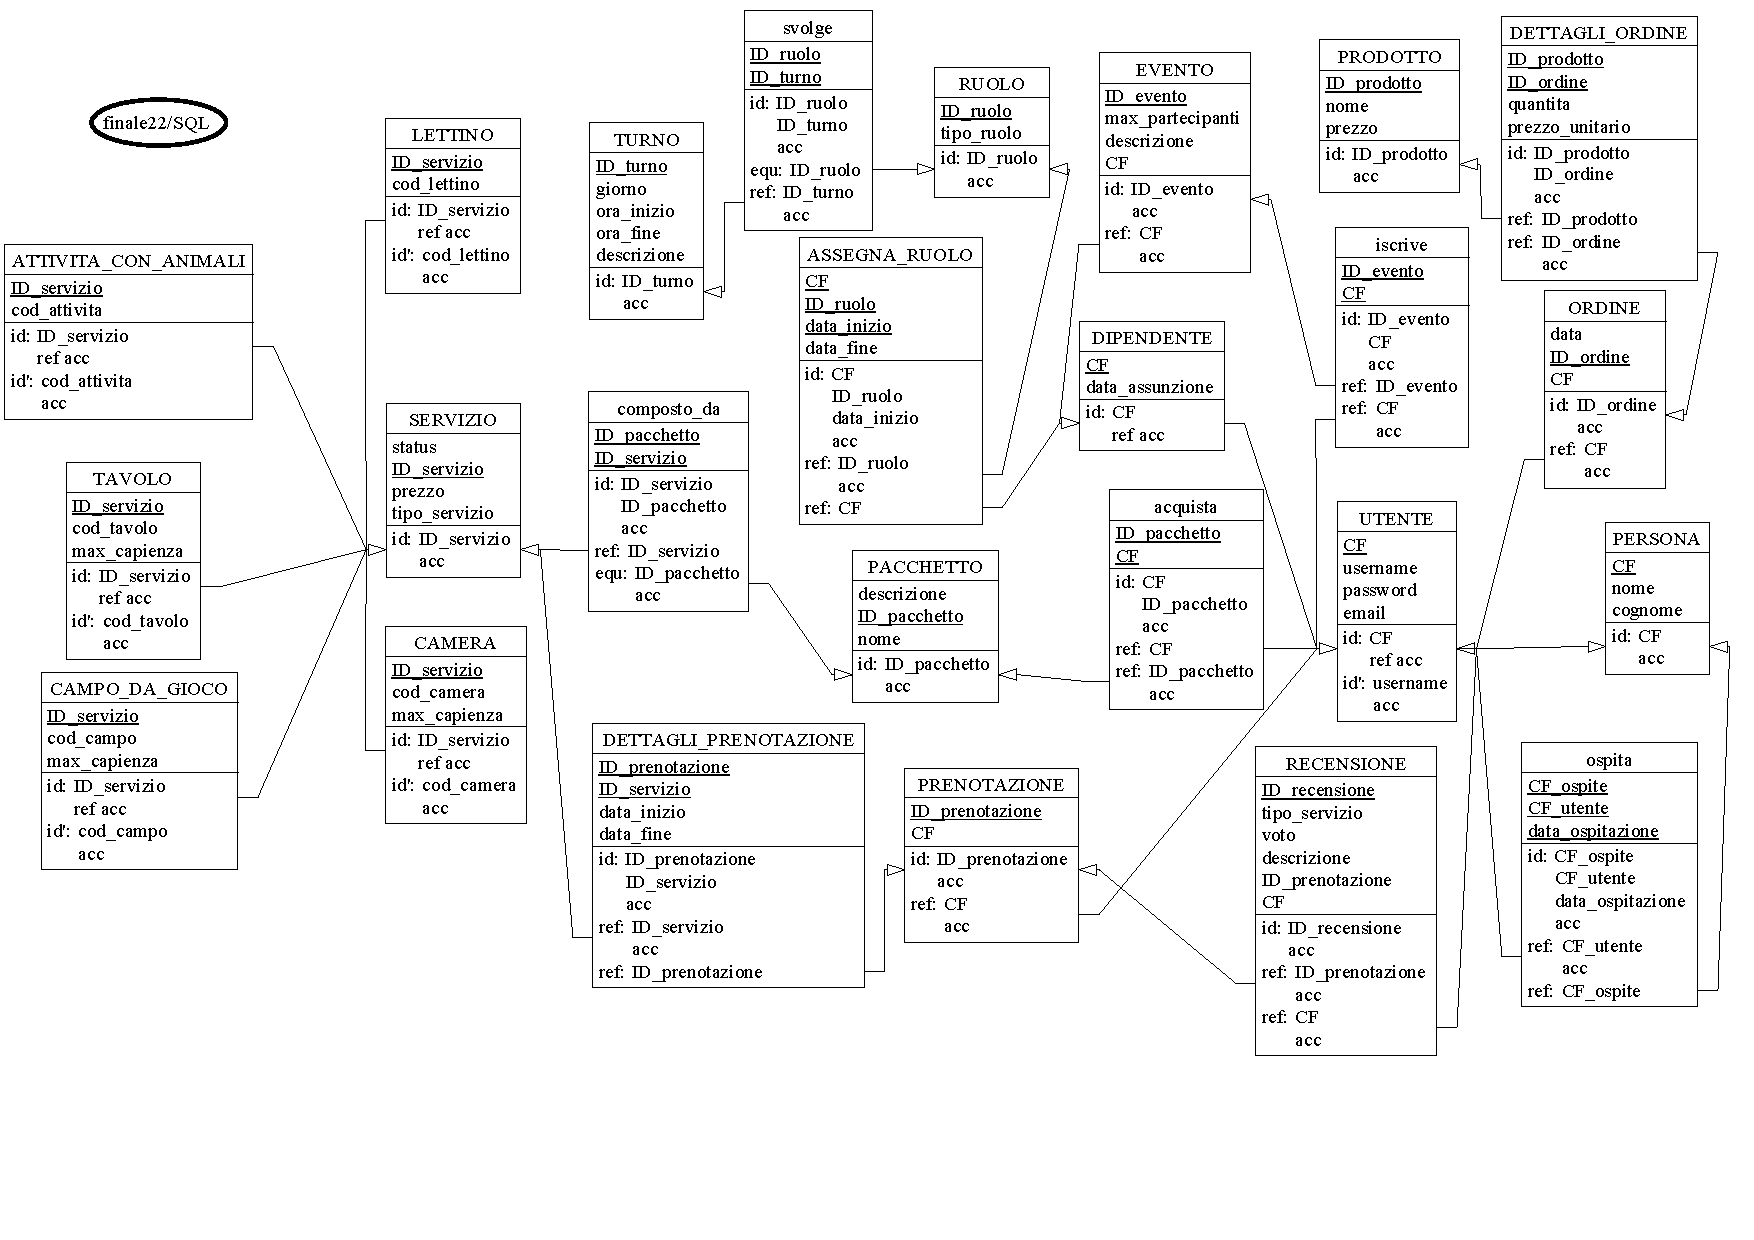
\includegraphics[width=\textwidth, trim=0 75pt 120pt 0 , clip]{./pdf/finale logico.pdf}
	\caption{Schema logico, schema relazionale finale}
	\label{fig:schema-logico}
\end{figure}
\subsection{Schema relazionale (grafico)}

\subsection{Schema relazionale (testuale)}
Di seguito viene riportata la traduzione in schema relazionale delle entità e relazioni progettate.
Le chiavi primarie sono indicate con attributi sottolineati; le chiavi esterne sono sottolineate e seguite da ``: NOME\_TABELLA''.

\begin{description}
	\item\texttt{\textbf{UTENTE} \\
		      (\underline{username}, password, email)}
	\item\texttt{\textbf{PERSONA} \\
		      (\underline{CF}, nome, cognome)}
	\item\texttt{\textbf{DIPENDENTE} \\
		      (\underline{CF} : PERSONA, data\_assunzione)}
	\item\texttt{\textbf{RUOLO} \\
		      (\underline{ID\_ruolo}, tipo\_ruolo)}
	\item\texttt{\textbf{ASSEGNA\_RUOLO} \\
		      (\underline{CF} : DIPENDENTE, \underline{ID\_ruolo} : RUOLO, \underline{data\_inizio}, data\_fine)}
	\item\texttt{\textbf{SERVIZIO} \\
		      (\underline{ID\_servizio}, tipo\_servizio, prezzo, status)}
	\item\texttt{\textbf{RECENSIONE} \\
		      (\underline{ID\_recensione}, voto, descrizione, tipo\_servizio, \underline{username} \newline : UTENTE, \underline{ID\_servizio} : SERVIZIO)}
	\item\texttt{\textbf{PRODOTTO} \\
		      (\underline{ID\_prodotto}, nome, prezzo)}
	\item\texttt{\textbf{ORDINE} \\
		      (\underline{ID\_ordine}, data, \underline{username} : UTENTE)}
	\item\texttt{\textbf{DETTAGLI\_ORDINE} \\
		      (\underline{ID\_ordine} : ORDINE, \underline{ID\_prodotto} : PRODOTTO, quantita, \newline prezzo\_unitario, prezzo)}
	\item\texttt{\textbf{PRENOTAZIONE} \\
		      (\underline{ID\_prenotazione}, \underline{username} : UTENTE)}
	\item\texttt{\textbf{DETTAGLI\_PRENOTAZIONE} \\
		      (\underline{ID\_prenotazione} : PRENOTAZIONE, \underline{ID\_servizio} : SERVIZIO, \newline \underline{data\_inizio}, data\_fine)}
	\item\texttt{\textbf{PACCHETTO} \\
		      (\underline{ID\_pacchetto}, nome, descrizione)}
	\item\texttt{\textbf{EVENTO} \\
		      (\underline{ID\_evento}, descrizione, max\_partecipanti)}
	\item\texttt{\textbf{TAVOLO} \\
		      (\underline{cod\_tavolo}, max\_capienza)}
	\item\texttt{\textbf{CAMERA} \\
		      (\underline{cod\_camera}, max\_capienza)}
	\item\texttt{\textbf{LETTINO} \\
		      (\underline{cod\_lettino})}
	\item\texttt{\textbf{CAMPO\_DA\_GIOCO} \\
		      (\underline{cod\_campo}, max\_capienza)}
	\item\texttt{\textbf{ATTIVITA\_CON\_ANIMALI} \\
		      (\underline{cod\_attivita})}
\end{description}

\chapter{Progettazione della Base di Dati}
Ora che abbiamo creato la nostra base di dati, mappiamo le nostre realzioni in tabelle, per poi utilizzarle nel nostro

\section{Traduzione delle operazioni}

\chapter{Progettazione dell'applicazione}


\end{document}
